\documentclass[12pt, a4paper]{article}

\usepackage[utf8]{inputenc}
\usepackage[russian]{babel}
\usepackage[OT1]{fontenc}
\usepackage{amsfonts}
\usepackage{amsmath}
\usepackage{amssymb}
\usepackage{amsthm}
\usepackage{mathrsfs}
\usepackage{mathtools}
\usepackage{fancyhdr}
\usepackage{fancybox}
	\cornersize{1}
\usepackage{tikz}
	\usetikzlibrary{arrows,decorations.pathmorphing,backgrounds,positioning,fit,petri}
\usepackage{cancel}

\usepackage{enumitem}
\setlist[enumerate]{itemsep=1pt, label={\arabic*.}, leftmargin=1.3pc}

\usepackage[left = 3cm, right = 3cm, top = 3cm, bottom = 4cm, a4paper]{geometry}
\usepackage{geometry}

\usepackage{graphicx}
\usepackage{subcaption}
\usepackage{wrapfig}
\graphicspath{{./img/}}

\newtheorem*{exersize}{Упражнение}
\newtheorem*{lemma}{Лемма}
\newtheorem*{theorem}{Теорема}
\newtheorem*{consequence}{Следствие}
\newtheorem*{statement}{Утверждение}
\newtheorem{property}{Свойство}
\newtheorem*{fact}{Факт}

\theoremstyle{definition}
\newtheorem*{definition}{Определение}
\newtheorem*{problem}{Задача}
\newtheorem*{example}{Пример}

\theoremstyle{remark}
\newtheorem*{note}{Замечание}

\renewcommand{\qedsymbol}{{\footnotesize$\blacksquare$}}

\makeatletter
  \renewenvironment{proof}[1][\proofname]{\par
    \pushQED{\qed}%
    \normalfont \topsep6\p@\@plus6\p@\relax
    \trivlist
    \item\relax
          {$\blacktriangle$}\hspace\labelsep\ignorespaces
  }{%
    \popQED\endtrivlist\@endpefalse
  }
  \makeatother

\renewcommand{\thesection}{\arabic{section}\hskip-12pt}
\renewcommand{\thesubsection}{}


\title{Конспект лекций по курсу\\ <<Теория вероятностей>>}
\author{Лектор: к. ф.-м. н. Родионов Игорь Владимирович}
\date{Набор: Алексей Шепелев, Александр Валентинов,\\ Василий Морковкин}

\usepackage{hyperref}
\hypersetup{
    colorlinks,
    citecolor=black,
    filecolor=black,
    linkcolor=black,
    urlcolor=black
}

\pagestyle{fancy}
\fancyhf{}
\fancyhead[L]{\hyperlink{page.1}{Конспект лекций по курсу <<Теория вероятностей>>}}
\fancyhead[R]{Лекция \thesection\kern1em}
\renewcommand{\headrulewidth}{0.5pt} 
\renewcommand{\footrulewidth}{0.5pt}
\fancyfoot{} 
\fancyfoot[C]{\thepage}



\renewcommand{\P}{\mathsf{P}}
\newcommand{\E}{\mathsf{E}}
\newcommand{\D}{\mathsf{D}}
\newcommand{\B}{\mathscr{B}}
\newcommand{\R}{\mathbb{R}}
\newcommand{\N}{\mathbb{N}}
\newcommand{\Z}{\mathbb{Z}}
\newcommand{\F}{\mathcal{F}}
\renewcommand{\G}{\mathcal{G}}
\newcommand{\M}{\mathcal{M}}
\DeclareMathOperator{\cov}{cov}
\DeclareMathOperator{\var}{Var}
\DeclareMathOperator{\const}{const}
\DeclareMathOperator{\rg}{const}
\newcommand{\indep}{\!\perp\!\!\!\!\perp\!}
\newcommand{\limn}{\xrightarrow[n \rightarrow + \infty]{}}

\setlength{\parindent}{0pt}
\setlength{\parskip}{3pt}

%\binoppenalty=\maxdimen
%\relpenalty=\maxdimen



\begin{document}
	\maketitle
	\tableofcontents
	\section{Лекция от 10.02.2018}
Будем обозначать вероятностное пространство как $(\Omega,  \F, \P)$, где 
\begin{enumerate}
	\item $\Omega$~--- пространство элементарных исходов;
	\item $\F$~--- $\sigma$-алгебра на $\Omega$;
	\item{$\P: \F \rightarrow [0, 1]$~--- вероятностная мера, причем
		\begin{enumerate}
			\item[a)] $\P (\Omega) = 1$;
			\item[b)] $\P$~--- $\sigma$-аддитивна, то есть $\forall \{A_n\}_{n = 1}^{+\infty} \in \F$, причем $A_n \cap A_m = \varnothing$ при $n \neq m$: $\P \left( \bigsqcup\limits_{n=1}^{+\infty} A_n \right) = \sum \limits_{n = 1}^{+\infty} \P (A_n)$.
		\end{enumerate}
	}
\end{enumerate}
\begin{definition}
	Последовательность $\{A_n\}$ убывает к $A$, если $\forall n: A_{n} \supseteq A_{n+1}$ и   $A = \bigcap\limits_{n = 1}^{+\infty} A_n$. Последовательность $\{A_n\}$ возрастает к $A$, если $\forall n: A_{n} \subseteq A_{n+1}$ и   $A = \bigcup\limits_{n = 1}^{+\infty} A_n$.
\end{definition}
\begin{theorem}[о непрерывности вероятностной меры][б/д]
	Пусть $(\Omega, \F )$~--- измеримое пространство и на нем определена функция $\P : \F \rightarrow [0,1]$, удовлетворяющая следующим свойствам: $\P (\Omega) = 1$ и $\P$~--- конечно аддитивная. Тогда следующие утверждения эквивалентны:
	\begin{enumerate}
		\item $\P$~--- вероятностная мера;
		\item $\forall A_n \downarrow A: \P (A_n) \rightarrow \P(A)$ (непрерывность снизу);
		\item $\forall A_n \uparrow A: \P (A_n) \rightarrow \P(A)$ (непрерывность сверху);
		\item  $\forall A_n \downarrow \varnothing: \P (A_n) \rightarrow 0$ (непрерывность в нуле).
	\end{enumerate}
\end{theorem}
\begin{theorem}[Каратеодори][б/д]
	Пусть $\Omega$~--- некое множество, $\mathcal{A}$~--- алгебра на $\Omega$ и $\P_\sigma$~--- вероятностная мера на $(\Omega, \mathcal{A})$. Тогда существует единственная вероятностная мера на $\big(\Omega, \sigma(\mathcal{A}) \big)$, являющаяся продолжением $\P_\sigma$, то есть  $ \forall A \in \mathcal{A}: \P_\sigma(A) = \P(A)$.
\end{theorem}

\subsection{Функция распределения}

Рассмотрим измеримое пространство $\big(\R, \B(\R)\big)$ и вероятностную меру $\P$~на~нем.
\begin{definition}
	Функция $F(x), x \in \R$, заданная по правилу $F(x) = \P \big( (-\infty, x] \big)$~--- функция распределения вероятностной меры  $\P$.
\end{definition}
\begin{lemma}[свойства функции распределения]
	Пусть $F(x)$~--- функция распределения, тогда
	\begin{enumerate}
		\item $F(x)$ не убывает;
		\item $\lim\limits_{x \rightarrow +\infty} F(x) = 1$; $\lim\limits_{x \rightarrow -\infty} F(x) = 0$;
		\item $F(x)$ непрерывна справа.
	\end{enumerate}
	\begin{proof}
		Пусть $y \geqslant x$, тогда $F(y) - F(x) = \P \big( (-\infty, y] \big) - \P \big( (-\infty, x] \big) = \P \big( (x, y] \big) \geqslant 0$, следовательно, $F(x)$ неубывает.
		
		Пусть $x_n \rightarrow -\infty$ при $n \rightarrow +\infty$, тогда $(-\infty, x_n] \rightarrow \varnothing$, следовательно, $F(x_n) = \P \big( (-\infty, x_n] \big) \underset{n \rightarrow +\infty}{\longrightarrow} 0$ по теореме о непрерывности вероятностной меры. 
		
		Пусть $x_n \rightarrow +\infty$ при $n \rightarrow +\infty$, тогда $(-\infty, x_n] \rightarrow \R$, следовательно, $F(x_n) = \P \big( (-\infty, x_n] \big) \underset{n \rightarrow +\infty}{\longrightarrow} \P(\R) = 1$.
				
		Пусть $x_n \downarrow x$, тогда $(-\infty, x_n] \downarrow (-\infty, x]$, отсюда по теореме о непрерывности вероятностной меры вытекает, что $F(x_n) = \P \big( (-\infty, x_n] \big) \underset{n \rightarrow +\infty}{\longrightarrow} \P \big( (-\infty, x] \big) =~F(x)$.
	\end{proof}
\end{lemma}
\begin{property}
	Функция распределения имеет предел слева $\forall x \in \R$, при этом число точек разрыва не более, чем счетно.
	\begin{proof}
		Пусть $x_n \rightarrow x - 0$~--- возрастающая последовательность, тогда $F(x_n) = \P \big( (-\infty, x_n] \big) \underset{n \rightarrow +\infty}{\longrightarrow} \P \big( (-\infty, x) \big) = F(x - 0)$. Каждая точка разрыва~--- скачок функции распределения, каждому скачку сопоставим $[F(x-0), F(x)]$, а этому отрезку в свою очередь сопоставим некую рациональную точку, которая лежит в $(F(x-0), F(x))$. Следовательно каждому скачку мы сопоставили точку из $\mathbb{Q}$, а так как $\mathbb{Q}$ счетно, то число разрывов не более, чем счетно.
	\end{proof}
\end{property}
\begin{definition}
	Функция $F(x)$, которая удовлетворяет свойствам 1) -- 3) из леммы, называется функцией распределения на $\R$.
\end{definition}
\begin{theorem}[о взаимно однозначном соответствии между вероятностной мерой и функцией распределения на $\R$]
	Пусть $F(x)$~--- функция распределения на $\R$, тогда существует единственная вероятностная мера $\P$ на $\big(\R, \B(\R) \big)$ такая, что $F(x)$ является ее функцией распределения, то есть $F(x) = \P \big( ( -\infty, x] \big)$.
	\begin{proof}
		Рассмотрим полукольцо $ S = \big\{ (a, b] \big\}$ на $\R$. Определим $\sigma$-аддитивную вероятностную меру $\P \big( (a, b] \big) = F(b) - F(a)$, а по теореме Каратеодори $\P$ единственным образом продолжается на всю $\sigma$-алгебру $\B(\R)$.
	\end{proof}
\end{theorem}
\subsection{Классификация вероятностных мер и функций распределения на прямой}
\subsubsection*{\ovalbox{1}~~Дискретное распределение}
Пусть $\mathscr{X} \subseteq \R$ не более, чем счетно.
\begin{definition}
	Вероятностная мера $\P$ на $\big( \R, \B(\R) \big)$, удовлетворяющая свойству $\P(\R \backslash \mathscr{X}) = 0$, называется дискретной вероятностной мерой на $\mathscr{X}$, ее функция распределения также называется дискретной.
\end{definition}

Рассмотрим $\mathscr{X} = \{ x_k \}$, положим $p_k = \P \big( \{x_k \} \big)$, тогда $\P( \mathscr{X} ) = 1 = \sum\limits_{k} \P ( x_k )$.

\begin{definition}
	Набор чисел $\{ p_k \}$ на называется распределением вероятностей на $\mathscr{X}$.
\end{definition}

\subsubsection*{\ovalbox{2}~~Абсолютно непрерывное распределение}
\begin{definition}
	Пусть $F(x)$~--- функция распределения вероятностной меры $\P$ на $\R$, причем $\forall x \in \R$ верно $F(x) = \int\limits_{-\infty}^{x} p(t) \, d t$, где  $p(t) \geqslant 0$, а $\int\limits_{-\infty}^{+\infty} p(t) \, d t = 1$. Тогда $\P$ абсолютно непрерывна, $F(x)$ также называется абсолютно непрерывной, а $p(t)$~--- плотность распределения $F(x)$. Причем $p(t)$ определена однозначно, кроме множества меры нуль.
\end{definition}
\noindent {\bfseries Примеры:}
\begin{enumerate}
	\item{ Равномерное распределение $R[a,b]$ 
		$$p(x) = \frac{1}{b -a } \cdot I \big( x \in [a,b] \big). $$}
	\item{Нормальное (гауссовское) распределение $N(a, \sigma^2)$
		$$p(x) = \frac{1}{\sqrt{2 \pi \sigma^2}} \cdot \exp \left[ -\frac{(x - a)^2}{2 \sigma^2} \right]. $$}
	\item{Экспоненциальное распределение $\text{Exp}(\alpha)$
	$$p(x) = \alpha e^{-\alpha x} \cdot I(x > 0).$$}
	\item{Распределение Коши $\text{Cauchy}(\theta)$
		$$p(x) = \frac{\theta}{\pi \left(x^2 + \theta^2 \right)}.$$}
	\item{ Гамма распределение $\Gamma(\alpha, \gamma)$
		$$p(x) = \frac{x^{\alpha - 1} \gamma^{\alpha}}{\Gamma(\alpha)} \cdot e^{-\gamma x} \cdot I(x > 0).$$}
\end{enumerate}
\begin{definition}
	$\Gamma(\alpha) = \int\limits_0^{+\infty} x^{\alpha - 1} e^{-x} \, d x$, причем $\forall n \in \N : \Gamma(n) = (n - 1)!$, $\forall \lambda \in \R: \Gamma(\lambda \pm 1) = \lambda \Gamma(\lambda)$, а $\Gamma\left(\dfrac{1}{2}\right) = \sqrt{\pi}$.
\end{definition}
\subsubsection*{\ovalbox{3}~~Сингулярные распределения}
\begin{definition}
	Пусть $F(x)$~--- функция распределения на $\R$. Точка $x_0 \in \R$ называется точкой роста $F(x)$, если $\forall \varepsilon > 0: F(x_0 + \varepsilon) - F(x_0 - \varepsilon) > 0$.
\end{definition}
\begin{definition}
	Функция распределения называется сингулярной, если она непрерывна и множество ее точек роста имеет Лебегову меру нуль. Например, функция Кантора.
\end{definition}
\begin{theorem}[Лебега о функции распределения][б/д]
	Пусть $F(x)$~--- функция распределения на $\R$. Тогда существуют единственные $\alpha_1, \alpha_2$ и $\alpha_3$, $\alpha_i \geqslant 0, \alpha_1 + \alpha_2 + \alpha_3 = 1$ и функции распределения $F_1(x), F_2(x)$ и $F_3(x)$ такие, что $F(x) = \alpha_1 F_1(x) + \alpha_2 F_2(x) + \alpha_3 F_3(x)$, где $F_1(x)$~--- дискретная функция распределения, $F_2(x)$~--- абсолютно непрерывная, а $F_3(x)$~--- сингулярная. 
\end{theorem}
	\section{Лекция от 17.02.2018}
\subsection{Вероятностная мера в $\big( \R^n, \B(\R^n) \big)$}
\begin{definition}
	Пусть $\P$~--- вероятностная мера в $\big( \R^n, \B(\R^n) \big)$, тогда функция $F(\vec x) = \P\big((-\infty; x_1] \times \ldots \times (-\infty, x_n]\big)$ называется функцией распределения вероятностной меры $\P$ в $\R^n$.
\end{definition}
\begin{note}
	Пусть $\vec x^{(k)} = \left(x_1^{(k)}, \ldots, x_n^{(k)}\right) \in \R^n$. Будем писать $\vec x^{(k)} \downarrow \vec x$, если $\forall i, k : x_i^{(k)} \geqslant x_i^{(k + 1)}$ и $x_i^{(k)} \underset{k \rightarrow +\infty}{\longrightarrow} x_i$.
\end{note}
\begin{lemma}[Свойства многомерной функции распределения]
	Пусть $F(\vec x)$~--- функция распределения вероятностной меры в $\R^n$, тогда
	\begin{enumerate}
		\item Если $\vec x^{(k)} \downarrow \vec x$, то $F\big(\vec x^{(k)}\big) \rightarrow F\big(\vec x\big), k \rightarrow +\infty$;
		\item $\lim\limits_{\forall i : x_i \rightarrow +\infty} F(\vec x) = 1;\; \lim\limits_{\exists i : x_i \rightarrow -\infty} F(\vec x) = 0$;
		\item $\forall a_1 < b_1, a_2 < b_2, \ldots,\;\; \Delta_{a_1b_1}^1 \ldots \Delta_{a_nb_n}^nF(x) > 0 :$, где \\
		$\Delta_{a_ib_i}^i F(\vec x) = F(x_1, \ldots, x_{i - 1}, b_i, x_{i + 1}, \ldots x_n) - F(x_1, \ldots, x_{i - 1}, a_i, x_{i + 1}, \ldots, x_n)$.
	\end{enumerate}
	\begin{proof}
		Первое свойство следует из непрерывности вероятностной меры, так как $\bigtimes\limits_{i = 1}^n\big(-\infty, x_i^{(k)}\big] \downarrow \bigtimes\limits_{i = 1}^n \big(-\infty, x_i\big]$. \\
		\medskip
		
		$B_n \curvearrowright C_n = \bigtimes\limits_{i = 1}^n\big(-\infty, \inf\limits_{k \geqslant n} x_i^{(k)}\big] \\
		\P(B_n) \rightarrow \P(\R^n) = 1$ \\
		Если $\exists i : x_i^{(k)} \rightarrow - \infty$, то $B_n \rightarrow \varnothing, \P(B_n) \rightarrow 0$;
		\medskip
		
		$\Delta_{a_1b_1}^1 \ldots \Delta_{a_nb_n}^nF(x) = \P\big((a_1, b_1] \times \ldots \times (a_n, b_n]\big)$ \\
		$\Delta_{a_1b_1}^1\Delta_{a_2,b_2}^2F(x) = F(b_1,b_2) - F(a_1,b_2) - (F(b_1,a_2) - F(a_1,a_2))$
	\end{proof}
\end{lemma}
\begin{theorem}[О взаимооднозначном соответствии вероятностной меры и функции распределения в $\R^n$][б/д]
	Если функция $F(\vec x),\; \vec x \in \R^n$ удовлетворяет свойствам из леммы, то существует единственная $\P$ в $\R^n$, для которой $F(\vec x)$ является функцией распределения.
\end{theorem}
\begin{note}
	Почему нельзя заменить свойство 3) на монотонность на любом компакте? 
	\begin{proof}
		Пусть $F(x_1, x_2) = \max(x_1, x_2)$ на $[0, 1]^2$, но тогда $-1 = \Delta_{0; 1}^1 \Delta_{0; 1}^2 F(x_1, x_2) \neq \P([0, 1]^2) = 1$. Следовательно, $F(x)$ не функция распределения.
	\end{proof}
\end{note}
\begin{definition}
	Функция $F(\vec x)$, удовлетворяющая условиями из леммы называется функцией распределения в $\R^n$.
\end{definition}
\subsection{Многомерная плотность вероятности}
\begin{definition}
	Если 
	$$ F(x_1, \ldots, x_n) = \int\limits_{-\infty}^{x_1}\ldots\int\limits_{-\infty}^{x_n} p(y_1, \ldots, y_n)dy_1\ldots dy_n,\; p(x_1, \ldots, x_n) \geqslant 0, $$ 
	то $p(x_1, \ldots, x_n)$ называется $n$-мерной плотностью вероятности. Тогда
	$$ p(x_1, \ldots, x_n) = \frac{\partial^n}{\partial x_1\ldots\partial x_n}F(x_1, \ldots, x_n). $$
\end{definition}
\subsection{Случайные величины}
\begin{definition}
	Пусть $\big(\Omega, \F \big)$ и $\big( E, \mathcal{E} \big)$~--- два измеримых пространства. Отображение $X: \Omega \rightarrow E$~--- случайный элемент, если $\forall B \in \mathcal{E}: X^{-1} \in \F$ $\F$-измеримо или $\F|\mathcal{E}$-измеримо. \\
	Если $(E, \mathcal{E}) = \big(\R, \B(\R)\big)$, то это случайная величина. \\
	Если $(E, \mathcal{E}) = \big(\R^n, \B(\R^n)\big)$, то это случайный вектор.
\end{definition}
\subsection{Действия над случайными величинами и векторами}
\begin{definition}
	Функция $\varphi: \R^n \rightarrow \R^m$~--- борелевская, если $\forall B \in \B(\R^m): \varphi^{-1}(B) \in \B(\R^n)$. 
\end{definition}
\begin{statement}
	Любая непрерывная и кусочно-непрерывная функция~--- борелевская.
\end{statement}
\begin{theorem}[критерий измеримости][б/д]
	Пусть $\big(\Omega, \F\big), \big(E, \mathcal{E}\big)$~--- два измеримых пространства, $X: \Omega \rightarrow E$~--- случайный элемент тогда, и только тогда, когда существует система событий $\M \subseteq \mathcal{E}$, такая что $\sigma(\M) = \mathcal{E}$ и $\forall B \in \M: X^{-1}(B) \in \F$.
\end{theorem}
\begin{lemma}
	Пусть $\vec\xi = (\xi_1, \ldots, \xi_n)$~--- случайный вектор, $\varphi: \R^n \rightarrow \R^m$~--- борелевская функция, тогда $\varphi(\vec\xi)$~--- случайный вектор.
	\begin{proof}
		Пусть $B \in \B(\R^n)$. Тогда 
		$$ (\varphi(\vec\xi))^{-1}(B) = \big\{\omega : \varphi(\vec\xi(\omega)) \in B\big\} = \big\{\omega : \vec\xi(\omega) \in \varphi^{-1}(B) \subseteq \B(\R^n) \big\} \in \F. $$
	\end{proof}
\end{lemma}
\begin{lemma}
	$\vec \xi = (\xi_1, \ldots, \xi_n)$~--- случайный вектор тогда, и только тогда, когда $\forall i : \xi_i$~--- случайная величина.
	\begin{proof}
		\emph{Необходимость.} $\varphi(x_1, \ldots, x_n) = x_i$~--- непрерывная функция, значит борелевская, следовательно, по предыдущей лемме $\xi_i$~--- случайная величина. \\
		\emph{Достаточность.} $\B(\R^n) = \sigma\big(B_1 \times \ldots \times B_n, B_i \in \B(\R)\big)$, поэтому $\vec\xi^{-1}(B_1 \times \ldots \times B_n) = \big\{\omega : \vec\xi(\omega) \in B_1 \times \ldots \times B_n\big\} = \big\{\omega : \xi_1(\omega) \in B_1, \ldots, \xi_n(\omega) \in B_n\big\} = \bigcap\limits_{i = 1}^n\big\{\omega: \xi(\omega) \in B_i \big\} = \bigcap\limits_{i = 1}^n \xi_i^{-1}(B_i) \in \F$, значит, по критерию измеримости, $\vec \xi$~--- случайный вектор.
	\end{proof}
\end{lemma}
\begin{consequence}
	Пусть $\xi$, $\eta$~--- случайные величины, $c \in \R$,тогда $\xi + \eta$, $\xi - \eta$, $c\xi$, $\xi \cdot \eta$ и $\xi / \eta$, если $\forall \omega \in \Omega : \eta \neq 0$ тоже случайные величины.
\end{consequence}
\begin{lemma}[О пределах случайной величины]
	Пусть $\big\{ \xi_n, n \in \N \big\}$ последовательность случайных величин, тогда, если пределы $\overline{\lim}~\xi_n$, $\underline{\lim}~\xi_n$, $\inf\xi_n$, $\sup\xi_n$ существуют, они являются случайными величинами.
	\begin{proof}
		$\big\{\omega : \sup \xi_n \leqslant x \big\} = \bigcap\limits_{n = 1}^{+\infty}\big\{\omega : \xi_n(\omega) \leqslant x \big\} \in \F$. По критерию измеримости, так как $\sigma\big(x : (-\infty, x]\big) = \B(\R)$, мы доказали, что $\sup\xi_n$~--- случайная величина. Аналогично, $\big\{\omega : \inf \xi_n > x \big\} = \bigcup\limits_{k = 1}^{+\infty}\big\{\omega : \xi_n(\omega) \geqslant x \big\} \in \F$, так как $\sigma\big((x, +\infty)\big) = \B(\R)$, по критерию измеримости $\inf\xi_n$~--- случайная величина. Отсюда $\overline{\lim}~\xi_n = \inf\limits_n\sup\limits_{m \geqslant n}~\xi_m$ и $\underline{\lim}~\xi_n = \sup\limits_n\inf\limits_{m \geqslant n}~\xi_m$ тоже случайные величины.
	\end{proof}
\end{lemma}
\begin{consequence}
	Пусть $\xi = \lim \xi_n$ и предел существует $\forall \omega \in \Omega$, тогда $\xi$~--- случайная величина.
	\begin{proof}
	$\xi = \lim \xi_n = \overline{\lim}\xi_n = \underline{\lim} \xi_n$
	\end{proof}
\end{consequence}
\subsection{Характеристики случайных величин и векторов}
\subsubsection*{\ovalbox{1} Распределение случайной величины}
\begin{definition}
	Пусть $\big(\Omega, \F, \P \big)$~--- вероятностное пространство, $\xi$~--- случайная величина (вектор) на нем. Распределением случайной величины называется вероятностная мера $\P_\xi$ на $\big(\R, \B(\R)\big)$ $\big((\R^n, \B(\R^n))\big)$, заданная по правилу $\P_\xi(B) = \P(\xi \in B)$, $B \in \B(\R)$ ($B \in \B(\R^n)$).
\end{definition}
\subsubsection*{\ovalbox{2} Функция распределения случайной величины}
\begin{definition}
	Пусть $\big(\Omega, \F, \P\big)$~--- вероятностное пространство, $\xi$~--- случайная величина (вектор) на нем. Функцией распределения $\xi$ называется $F_\xi(x) = \P(\xi \leqslant x)$ ($F_\xi(\vec x) = \P(\xi_1 \leqslant x_1, \ldots, \xi_n \leqslant x_n)$).
\end{definition}
\subsubsection*{\ovalbox{3} Дискретность и непрерывность}
\begin{definition}
	Случайная величина называется дискретной, если ее распределение дискретно.
\end{definition}
\begin{definition}
	Случайная величина называется абсолютно непрерывной, если ее распределение абсолютно непрерывно, то есть $F_\xi(x) = \int\limits_{-\infty}^xp_\xi(y)dy,\; p_\xi(y) \geqslant 0$~--- плотность случайной величины $\xi$.
\end{definition}
\subsubsection*{\ovalbox{4} Сигма-алгебра, порожденная случайной величиной}
\begin{definition}
	Пусть $\xi$~--- случайная величина (вектор) на $\big(\Omega, \F, \P\big)$, тогда $\sigma$-алгеброй $\F_\xi$, порожденной случайной величиной $\xi$ называется $\F_\xi = \big\{\{\xi \in B\}, B \in \B(\R)\; (\in \B(\R^n)) \big\}$.
\end{definition}

	\section{Лекция от 03.03.2018}
\setcounter{property}{0}
\begin{definition}
	$\F = \big\{ \xi^{-1}(B), B \in \B(\R) \big\}$~--- порожденная $\sigma$-алгебра.
\end{definition}
\begin{definition}
	Пусть $\xi, \eta$~--- случайные величины. Тогда величина $\eta$ называется $\F_\xi$-измеримой, если $\F_\eta \subset \F_\xi$.
\end{definition}
\begin{example}
	Пусть $f$~--- борелевская, $\eta = f(\xi)$. Тогда $\eta$~--- $\F_\xi$-измерима.
	\begin{proof}
		$\{\eta \in B\} \in \F_\xi$, где $B \in \B(\R)$, значит $\{\eta \in B\} = \{\xi \in f^{-1}(B) \in \B(\R)\} \in~\F_\xi$
	\end{proof}
\end{example}
\begin{theorem}[][Пока б/д]
	Пусть  $\eta$~--- $\F_\xi$-измерима, тогда существует борелевская $\varphi$, такая что $\eta = \varphi(\xi)$ почти наверное, то есть $\P\big(\eta = \varphi(\xi)\big) = 1$.
\end{theorem}
\subsection{Независимость случайных величин}
\begin{statement}
Случайные величины независимы тогда, и только тогда, когда порождаемые ими $\sigma$-алгебры независимы.
\end{statement}
\begin{definition}
	Системы множеств $\F$ и $\G$ независимы, если $\forall A \in \F,\, B \in \G : \P(A \cap B) = \P(A)\cdot\P(B)$.
\end{definition}
\begin{definition}
	Пусть $\xi$ и $\eta$~--- случайные величины, тогда $\xi$ и $\eta$ независимы, если $\forall B_1, B_2 \in \B(\R) : \P(\xi \in B_1, \eta \in B_2) = \P(\xi \in B_1)\cdot\P(\eta \in B_2)$.
\end{definition}
\begin{definition}
	Случайные величины $\{\xi_i\}_{i = 1}^\infty$ независимы (в совокупности), если для любого конечного набора индексов $\alpha_1, \ldots, \alpha_n : \P(\xi_{\alpha_1} \in B_1, \ldots, \xi_{\alpha_n} \in B_n) = \prod\limits_{i = 1}^n\P(\xi_{\alpha_i} \in B_i),\; B_i \in \B(\R), i = 1, \ldots, n$.
\end{definition}
\begin{theorem}[Критерий независимости в терминах функции распределения]
	Случайные величины $\{\xi_i\}_{i = 1}^n$ независимы в совокупности тогда, и только тогда, когда $\forall x_1, \ldots, x_n \in \R : \P(\xi_1 \leqslant x_1, \ldots, \xi_n \leqslant x_n) = \prod\limits_{i = 1}^n\P(\xi_i \leqslant x_i)$.
	\begin{proof}
		Возьмем в качестве $B_i = (-\infty, x_i]$.
	\end{proof}
\end{theorem}
\begin{theorem}
	Пусть $(\xi_1, \ldots, \xi_n)$~--- независимые случайные векторы, $\xi_i$ имеет размерность $n_i$. Пусть $f_i: \R^{n_i} \rightarrow \R^{k_i}$~--- борелевские функции. Тогда величины $f_1(\xi_1), \ldots, f_n(\xi_n)$~--- независимые.
	\begin{proof}
		Обозначим $\eta_i = f_i(\xi_i) \Rightarrow \eta_i$~--- $\F_{\xi_i}$-измеримая. По условию $\{\F_{\xi_i}\}_{i = 1}^\infty$~--- независимые $\sigma$-алгебры, следовательно $\{\F_{\eta_i}\}$ независимы, т.к. $\forall i : \F_{\eta_i} \subset \F_{\xi_i}$, значит по определению $\{\eta_i\}$ независимы в совокупности.
	\end{proof}
\end{theorem}
\subsection{Интеграл Лебега}
\begin{lemma}[][б/д]
	$\forall \xi \geqslant 0$ существует набор простых случайных величин $\xi_n$: $\xi_n \uparrow \xi$ ($\xi_n$~--- простая, если $\xi_n = \sum\limits_{i = 1}^k c_iI_{A_i}$).
\end{lemma}
\begin{definition}
	Пусть $\xi$~--- простая случайная величина, то есть $\xi = \sum\limits_{i = 1}^k c_iI_{A_i}$, тогда матожидание $\E \xi = \sum\limits_{i = 1}^k c_i\P(A_i)$, где $\bigsqcup A_i = \Omega$.
\end{definition}
\begin{definition}
	Пусть $\xi \geqslant 0$, тогда матожидание $\E \xi = \lim\limits_{n \rightarrow \infty} \E \xi_n$, где $\xi_n \uparrow \xi$, $\xi_n$~--- простые неотрицательные случайные величины или $\E \xi = \sup\limits_{\eta \leqslant \xi}\E\eta$, $\eta$~--- простые неотрицательные. 
\end{definition}
\begin{definition}
	Пусть $\xi$~--- произвольные случайные величины. Пусть $\xi_+ = \max(\xi, 0)$, $\xi_- = \max(-\xi, 0) \Rightarrow \xi = \xi_+ - \xi_-$, тогда матожидание 
	$$ \E\xi =
		\begin{tabular}{|c|c|c|} \hline
		$\E\xi_- \setminus \E\xi_+$ & < $+\infty$ & = $+\infty$ \\ \hline
		$< +\infty$ & $\E\xi_+ - \E\xi_-$ & $+\infty$ \\ \hline
		$= +\infty$ & $-\infty$ & $\nexists$ \\ \hline
		\end{tabular}
	$$
\end{definition}
\begin{consequence}
	$\E \xi$~--- конечно $\Leftrightarrow \E|\xi|$~--- конечно.
	\begin{proof}
		$|\xi| = \xi_+ + \xi_-$. $E|\xi|$~--- конечно $\Leftrightarrow \E\xi_+, \E\xi_-$~--- конечны $\Leftrightarrow \E\xi$~--- конечно.
	\end{proof}
\end{consequence}
\subsection{Свойства матожидания}
\begin{property}
	Пусть $\xi$~--- случайная величина, $\E \xi$~--- конечно, тогда $\forall c \in \R : \E(c\xi)$~--- конечно и $\E(c\xi) = c\E\xi$.
	\begin{proof}
		Для простых случайных величин свойство очевидно. Пусть $\xi \geqslant 0$, $\xi_n \uparrow \xi$~--- последовательность простых неотрицательных случайных величин, $c \geqslant 0$. Тогда $c\xi_n \uparrow c\xi \Rightarrow \E(c\xi) = \lim\limits_{n \rightarrow \infty} \E(c\xi_n) = c \lim\limits_{n \rightarrow \infty} \E(\xi_n) = c\E\xi$. В общем случае $\xi = \xi_+ - \xi_-$, тогда $(c\xi)_+ = c\xi_+,\; (c\xi)_- = c\xi_- \Rightarrow \E(c\xi) = \E(c\xi)_+ - \E(c\xi)_- = c\E\xi$. Если $c < 0$, то $(c\xi)_+ = -c\xi_-$ и $(c\xi)_- = -c\xi_+$.
	\end{proof}
\end{property}
\begin{property}
	Если $\xi \leqslant \eta, \E \xi, \E \eta$~--- конечны, то $\E \xi \leqslant \E \eta$.
	\begin{proof}
		Для простых случайных величин~--- очевидно. Для неотрицательных $\xi$, $\eta$ $\E\xi = \sup\limits_{\mu \leqslant \xi}\E\mu$, где $\mu$~--- простая случайная величина. $\sup\limits_{\mu \leqslant \xi}\E\mu \leqslant \sup\limits_{\mu \leqslant \eta}\E\mu = \E\eta$. Пусть $\xi, \eta$~--- произвольные, тогда $\xi_+ \leqslant \eta_+$ и $\xi_- \geqslant \eta_-$. $\E\xi = \E\xi_+ - \E\xi_- \leqslant \E\eta_+ - \E\eta_- = \E\eta$.
	\end{proof}
\end{property}
\begin{property}
	Если $\E\xi$~--- конечно, то $|\E\xi| \leqslant \E|\xi|$.
	\begin{proof}
		$|\xi| = \xi_+ + \xi_- \Rightarrow E|\xi|$~--- конечно. $\underbrace{-\E\xi_+ - \E\xi_-}_{-\E|\xi|} \leqslant \underbrace{\E\xi_+ - \E\xi_-}_{\E_\xi} \leqslant \underbrace{\E\xi_+ + \E\xi_-}_{\E|\xi|}$.
	\end{proof}
\end{property}
\begin{property}[Аддитивность]
	Пусть $\xi$ и $\eta$~--- случайные величины, $\E\xi$ и $\E\eta$~--- конечные, тогда $\E(\xi + \eta) = \E(\xi) + \E(\eta)$.
	\begin{proof}
		Для простых случайных величин~--- очевидно. Пусть $\xi, \eta \geqslant 0$, возьмем $\xi_n \uparrow \xi$, $\eta_n \uparrow \eta$~--- простые и положительные. Тогда $\xi_n + \eta_n \uparrow \xi + \eta \Rightarrow \E(\xi + \eta) = \lim\limits_{n \rightarrow \infty}\E(\xi_n + \eta_n) = \lim\limits_{n \rightarrow \infty}\E \xi_n + \lim\limits_{n \rightarrow \infty} \E\eta_n = \E\xi + \E\eta$. Пусть $\xi, \eta$~--- произвольные, тогда $(\xi + \eta)_+ \leqslant \xi_+ + \eta_+$. Пусть $\delta = (\xi_+ + \eta_+) - (\xi + \eta)_+ \Rightarrow \E\delta + \E(\xi + \eta)_+ = \E\xi_+ + \E\eta_+ \Rightarrow \E(\xi + \eta)_+ = \E\xi_+ + \E\xi_- - \E\delta$. Аналогично, $\E(\xi + \eta)_- = \E\xi_- + \E\eta_- - \E\delta$. Тогда $\E(\xi + \eta) = \E(\xi + \eta)_+ - \E(\xi + \eta)_- = \E\xi_+ + \E\eta_+ - \E\delta - \E\xi_- - \E\eta_- + \E \delta = \E\xi + \E\eta$. Рассмотрим $(\xi + \eta)_- = (\xi + \eta)_+ - (\xi + \eta) = \xi_+ + \eta_+ - \delta - (\xi + \eta) = \xi_- + \eta_- - \delta$.
	\end{proof}
\end{property}
\begin{property}
	\begin{enumerate}
		\item Пусть $|\xi| \leqslant \eta$, $\E\eta$~--- конечное, тогда $\E \xi$~--- конечная.
		\item Пусть $\xi \leqslant \eta$, $\E\eta$~--- конечное, тогда $\E\xi < + \infty$. \\
		Пусть $\xi \geqslant \eta$, $\E\eta$~--- конечное, тогда $\E\xi > - \infty$.
		\item Если $\E\xi$~--- конечное и $A \in \F$, то $\E(\xi\cdot I_A)$~--- конечное.
	\end{enumerate}
	\begin{proof}
		\begin{enumerate}
			\item $\xi_-, \xi_+ \leqslant \eta \Rightarrow 0 \leqslant \E\xi_+ = \sup\limits_{0 \leqslant \mu \leqslant \xi_+}\E\mu = \E\eta < +\infty \Rightarrow \E\xi_+, \E\xi_- < +\infty \Rightarrow \E\xi$~--- конечное.
			\item $\xi_+ \leqslant \eta_+ < +\infty \Rightarrow$ по первому пункту $\E\xi_+ < +\infty \Rightarrow \E\xi < +\infty$.
			\item $(\xi\cdot I_A)_+ = I_A\cdot\xi_+ < \xi_+ \Rightarrow \E(\xi\cdot I_A)_+$~--- конечное. Аналогично $\E(\xi\cdot I_A)_-$~--- конечное $\Rightarrow \E(\xi\cdot I_A)$~--- конечное.
		\end{enumerate}
	\end{proof}
\end{property}
\begin{definition}
	Событие $A$ происходит почти наверное, если $\P(A) = 1$.
\end{definition}
\begin{property}
	Если $\xi = 0$ почти наверное, то $\E\xi = 0$.
	\begin{proof}
		Пусть $\xi$~--- простая случайная величина, то есть $\xi = \sum\limits_{k = 1}^nx_kI_{A_k}$, где $\{x_k\}$ различные, $\{A_k\}$~--- разбиение $\Omega$, $A_k = \{\xi = x_k\}$. Тогда если $x_k \neq 0$, то $A_k = \{\xi = x_k\} \subseteq \{\xi \neq 0\} \Rightarrow \P(A_k) \leqslant \P(\xi \neq 0) = 0 \Rightarrow \E\xi = \sum\limits_{k = 1}^n x_k\P(A_k) = 0$. Если $\xi \geqslant 0$, то $\E\xi = \sup\limits_{\xi \geqslant \eta} \E\eta$, где $\eta$~--- простые $\Rightarrow \E\xi \geqslant 0$. Но $0 \leqslant \eta \leqslant \xi = 0$ почти наверное $\Rightarrow \E\eta = 0 \Rightarrow \E\xi = 0$. Пусть $\xi$~--- произвольные $\Rightarrow \xi_+ = 0$ почти наверное, $\xi_- = 0$ почти наверное и $\E\xi = \E\xi_+ - \E\xi_- = 0.$
	\end{proof} 
\end{property}
	\section{Лекция от 10.03.2018}
\begin{property}
	Если $\xi = \eta$ почти наверное и $\E | \eta| < +\infty$, то $\E | \xi| < +\infty$ и $\E \xi = \E \eta$.
	\begin{proof}
		Пусть $A = \{ \xi \neq \eta \}$, тогда $I_A = 0$ почти наверное, следовательно $\xi \cdot I_a = 0$ почти наверное и $\eta \cdot I_A = 0$ почти наверное. Так как $\xi = \xi \cdot I_A + \xi \cdot I_{\overline A}$, то $\xi = \xi \cdot I_A + \eta \cdot I_A$, потому что на $\overline A$ выполняется $\xi = \eta$. Из свойства 6 имеем $\E \xi = \E ( \xi \cdot I_A ) + \E (\eta \cdot I_{\overline A} ) = \E ( \eta \cdot I_A) + E ( \eta \cdot I_{\overline A} ) = \E \eta$. 
	\end{proof}
\end{property}
\begin{property}
	Пусть $\xi \geqslant 0$ и $\E \xi = 0$, тогда $\xi = 0$ почти наверное.
	\begin{proof}
		Рассмотрим события $A = \{ \xi > 0 \}$ и $A_n = \left\{ \xi > \frac{1}{n} \right\} $, следовательно, $A_n \uparrow A$. Имеем $\P (A_n) = \E I_{A_n}$, так как $n\xi > 1$ на $A_n$, то  $\E I_{A_n} \leqslant \E (n\xi \cdot I_A) \leqslant n \E \xi = 0$, значит, $\P(A) = \lim\limits_{n \rightarrow +\infty} \P (A_n)$.
	\end{proof}
\end{property}
\begin{property}
	Пусть $\E \xi$ и $\E \eta$ конечны, $\forall A \in \F: \E (\xi \cdot I_A) \leqslant \E ( \eta \cdot I_A)$. Тогда  $\xi \leqslant \eta$ почти наверное.
	\begin{proof}
		Рассмотрим событие $B = \{ \xi > \eta \}$. Из условия и построения $B$ получаем, что $\E (\eta \cdot I_B) \leqslant \E (\xi \cdot I_B) \leqslant \E (\eta \cdot I_B)$, следовательно, $\E( \xi \cdot I_B) = \E(\eta \cdot I_B)$, значит $\E \big( (\xi - \eta) \cdot I_B \big) = 0$. Так как $(\xi - \eta) \cdot I_B \geqslant 0$, то по свойству 8 $(\xi - \eta) \cdot I_B = 0$ почти наверное, следовательно $I_B = 0$ почти наверное, потому что $\xi- \eta > 0$ на $B$.
	\end{proof}
\end{property}
\begin{theorem}[о математическом ожидании произвольной случайной величины]
	Пусть $\xi \indep \eta$, причем $\E \xi$ и $\E \eta$ конечны, тогда $\E \xi \eta$ конечно и $\E \xi \eta = \E \xi \cdot \E \eta$.
	\begin{proof}
		Пусть $\xi$ и $\eta$~--- простые случайные величины, то есть $\xi$ принимает значения $\{ x_1, \ldots, x_n \}$, $\eta$ принимает значения $\{ y_1, \ldots, y_n \}$. Тогда по линейности
		\begin{multline*}
			\E \xi \eta = \sum\limits_{k,j=1}^{n} x_k y_j \P (\xi = x_k, \eta = y_j) = \sum\limits_{k,j=1}^n x_k y_j \P(\xi = x_k) \cdot \P(\eta = y_j) = \\ = \sum\limits_{k = 1}^n x_k \P (\xi = x_k) \sum\limits_{j = 1}^{n} y_j \P (\eta = y_j) = \E \xi \cdot \E \eta.
		\end{multline*}
			
		Рассмотрим $\xi_n \uparrow \xi$, 
		$$\xi_n = \sum\limits_{k=0}^{n \cdot 2^n - 1} \dfrac{k}{2^n} I \left(\dfrac{k}{2^n} \leqslant \xi \leqslant \dfrac{k+1}{2^n} \right) + n I(\xi > n),$$
		 следовательно, $\xi_n = \varphi_n(\xi)$, значит, $\xi_n$~--- $\F_\xi$-измеримая. Пусть $\xi, \eta \geqslant 0$. Существует последовательность $\F_\xi$-измеримых ($\F_\eta$-измеримых) простых неотрицательных простых функций $\xi_n \uparrow \xi$ ($\eta_n \uparrow \eta$). Так как $\xi \indep \eta$, то $\xi_n = \varphi_n (\xi) \indep \varphi_n(\eta) = \eta_n$. Следовательно, $\xi_n \cdot \eta_n \uparrow \xi \cdot \eta$, а по определению математического ожидания $\E \xi\eta = \lim\limits_{n \rightarrow +\infty} \E (\xi_n \eta_n) =  \lim\limits_{n \rightarrow +\infty} \E \xi_n \cdot \E \eta_n = \E \xi \cdot \E \eta$.
			
		Пусть теперь $\xi$ и $\eta$~--- произвольные случайные величины. $\xi^+$ и $\xi^-$~--- функции от $\xi$, $\eta^+$ и $\eta^-$~--- функции от $\eta$, следовательно, $\xi^+ \indep \eta^+$ и $\xi^- \indep \eta^-$, отсюда $(\xi \eta)^+ = \xi^+ \eta^+ + \xi^- \eta^-$ значит, $\E (\xi \eta)^+ = \E \xi^+ \eta^+ + \E \xi^- \eta^- = \E \xi^+ \E \eta^+ + \E \xi^- \E \eta^-$, аналогично $\E (\xi \eta)^- = \E \xi^+ \eta^- + \E \xi^- \eta^+ = \E \xi^+ \E \eta^- + \E \xi^- \E \eta^+$. Осталось заметить, что $\E \xi \eta = \E (\xi \eta)^+ - \E ( \xi \eta)^- = \E \xi^+ \E \eta^+ + \E \xi^- \E \eta^- - \E \xi^+ \E \eta^- - \E \xi^- \E \eta^+ =  (\E \xi^+ - \E \xi^-) (\E \eta^+ - \E \eta^-) = \E \xi \cdot \E \eta$.
	\end{proof}
\end{theorem}
	
Пусть $\xi = \sum\limits_{i = 1}^n x_i \cdot I (\xi = x_i)$~--- простая случайная величина. Тогда $\E g(\xi) = \sum\limits_{i=1}^{n} g(x_i) \cdot \P(\xi = x_i) = \sum\limits_{i = 1}^n g(x_i) \Delta F_\xi (x_i)$, где $\Delta F_\xi(x_i) = F_\xi(x_i) - F_\xi (x_i - 0)$.

\begin{theorem}[о замене переменной в интеграле Лебега][б/д]
	Пусть $(\Omega, \F)$ и $(E, \mathcal{E})$~--- два измеримых пространства и $X = X(\omega)$~--- $\F | \mathcal{E}$-измеримая функция со значениями в $E$, то есть $\forall B \in \mathcal{E}: X^{-1}(B) \in \F$. Пусть $\P$~--- вероятностная мера на $(\Omega, \F)$ и $\P_X$~--- вероятностная мера на $(E, \mathcal{E})$, заданная по правилу $\P_X(A) = \P (\omega: X(\omega) \in A)$ для $A \in \mathcal{E}$. Тогда для любой $\mathcal{E}$-измеримой функции $g(x):E \rightarrow \R$, то есть $\forall B \in \B(\R): g^{-1}(B) \in \mathcal{E}$, верно, 
	$$\int\limits_A g(x) \P_X(dx) = \int\limits_{X^{-1}(A)} g\big( X(\omega) \big) \P(d \omega).$$
\end{theorem}

Пусть $\xi : \Omega \rightarrow \R (\R^n)$, в таком случае вероятностная мера $\P_\xi$ однозначно восстанавливается по $F_\xi$, следовательно, по теореме $\E g(\xi) = \int g(\xi) \, d\P = \int g(x) \P_\xi(dx) = \int g(x) \, d F_\xi (x)$.

Пусть  $\xi$~--- абсолютно непрерывная случайная величина с плотностью $p_\xi(x)$, тогда $d F_\xi (x) = p_\xi (x)$, следовательно $\E g(x) = \int\limits_{\R} g(x) p_\xi(x) \, d x$.

\subsection{Прямое произведение вероятностных пространств и формула свертки}

\begin{definition}
	Пусть $(\Omega_1, \F_1, \P_1)$ и $(\Omega_2, \F_2, \P_2)$~--- два вероятностных пространства. Тогда $(\Omega, \F, \P)$~--- их прямое произведение, если 
	\begin{enumerate}
		\item $\Omega = \Omega_1 \times \Omega_2$;
		\item $\F = \F_1 \otimes \F_2$, то есть $\F = \sigma\big\{ \{ B_1 \times B_2 \} | B_1 \in \F_1, B_2 \in \F_2 \big\}$;
		\item $\P = \P_1 \otimes \P_2$, то есть  $\P$~--- продолжение вероятностной меры $\P_1 \times \P_2$, заданное на прямоугольнике $B_1 \times B_2, B_1 \in \F_1, B_2 \in \F_2$ по правилу $\P(B_1 \times B_2) = \P_1 (B_1) \cdot \P_2 (B_2)$. Так как $\{B_1 \times B_2 \}$~--- полукольцо, то $\P$ существует и единственна по теореме Каратеодори.
	\end{enumerate}
\end{definition}
\begin{theorem}[Фубини][б/д]
	Пусть $(\Omega, \F, \P)$~--- прямое произведение вероятносных пространств $(\Omega_1, \F_1, \P_1)$ и $(\Omega_2, \F_2, \P_2)$. Пусть $\xi : \Omega \rightarrow \R$ такая, что $\int\limits_\Omega \big| \xi (\omega_1, \omega_2) \big| \, d \P < + \infty$. Тогда интегралы $\int\limits_{\Omega_1} \xi (\omega_1, \omega_2) \P_1 (d \omega_1)$ и $\int\limits_{\Omega_2} \xi(\omega_1, \omega_2) \P_2 (d \omega_2)$ определены почти наверное относительно $\P_2$ и $\P_1$ соответственно, являются измеримыми случайными величинами относительно $\F_2$ и $\F_1$, следовательно, 
	$$\int\limits_\Omega \xi (\omega_1, \omega_2) \, d \P = \int\limits_{\Omega_2} \int\limits_{\Omega_1} \xi (\omega_1, \omega_2) \P_1 (d \omega_1) \P_2 (d \omega_2) = \int\limits_{\Omega_1} \int\limits_{\Omega_2} \xi(\omega_1, \omega_2) \P_2 (d \omega_2) \P_1 (d \omega_1).$$
	 Из всего этого следует, что двойной интеграл равен повторному.
\end{theorem}
\begin{statement}
 	Пусть $\xi \indep \eta$~--- случайные величины, тогда $(\R^2, \B(\R^2), \P_{(\xi, \eta)}) = (\R, \B(\R), \P_\xi) \otimes (\R, \B(\R), \P_\eta)$.
 	\begin{proof} Достаточно проверить свойство прямого произведения:
 		\begin{enumerate}
 			\item $\R^2 = \R \times \R$;
 			\item $\B(\R^2) = \sigma(\B(\R) \times \B(\R))$ по определению борелевской $\sigma$-алгебры в $\R^2$;
 			\item $\P_{(\xi, \eta)} (B_1 \times B_2) = \P(\xi \in B_1, \eta \in B_2) = \P(\xi \in B_1) \cdot \P(\eta \in B_2) = \P_\xi(B_1) \cdot \P_\eta (B_2)$. \qedhere
 		\end{enumerate}
 	\end{proof}
\end{statement}
\begin{lemma}[о свертке]
	Пусть случайные величины $\xi$ и $\eta$ независимы c функциями распределения $F_\xi$ и $F_\eta$. Тогда
	$$ F_{\xi + \eta} (z) = \int\limits_\R F_\xi (z - x) \, dF_\eta (x) = \int\limits_\R F_\eta(z - x) \, d F_\xi(x).$$
	Если $\xi$ и $\eta$ имеют плотности распределения $f_\xi$ и $f_\eta$ соответственно, то $\xi + \eta$ имеет плотность распределения 
	$$f_{\xi + \eta} (z) = \int\limits_\R f_\xi (z - x) f_\eta (x) \, dx = \int\limits_\R f_\eta (z - x) f_\xi(x) \, dx$$.
	\begin{proof}
		Заметим, $F_{\xi + \eta} (z) = \P ( \xi + \eta \leqslant z)$, а по теореме о замене переменных в интеграле Лебега это равно $\int\limits_{\R^2} I(x + y \leqslant z) \P_\xi(dx) \P_\eta(dy)$, полученный двойной интеграл по Фубини можно записать как повторный:
		$$ \int\limits_\R \left( \int\limits_\R I(x + y \leqslant z) \P_\xi(dx) \right) \P_\eta(dy) = \int\limits_\R \left( \int\limits_{-\infty}^{z-y} \P_\xi(dx) \right) \P_\eta(dy) = \int\limits_\R F_\xi(z - y) \, dF_\eta(y).$$
		Перейдем ко второму пункту доказательства:
		\begin{multline*}
			F_{\xi + \eta} (z) = \int\limits_{\R^2} I(x + y \leqslant z) \P_\xi(dx) \P_\eta(dy) = \int\limits_{\R^2} I(x + y \leqslant z) f_\xi(x) f_\eta(y) \, dx\,dy \overset{t = x+y}{=} \\ \overset{t = x+y}{=} \int\limits_{\R^2} I(t \leqslant z) f_\xi(x) f_\eta(t - x) \, dx\,dt = \int\limits_{-\infty}^z \left( \int\limits_\R f_\xi(x) f_\eta(t-x) \, dx \right) \, dt.
		\end{multline*}
		Следовательно, по определению плотности, $f_{\xi+\eta} = \int\limits_\R f_\xi(x) f_\eta(t-x) \, dx$.
	\end{proof}
\end{lemma}
	\section{Лекция от 17.03.2018}
\subsection*{Дисперсия и ковариация}
\begin{definition}
	Дисперсией случайной величины $\xi$ называется $\D \xi = \E (\xi - \E \xi)^2 $, если $\E{\xi} < + \infty$. Очевидно, $\D{\xi} \geqslant 0$.
\end{definition}
\begin{definition}
	Ковариация двух случайных величин называется $\cov (\xi, \eta) = \E \big( ( \xi - \E \xi)(\eta - \E \eta ) \big)$. Легко заметить, что $\cov (\xi, \xi ) = \D \xi$. Если $\cov ( \xi, \eta) = 0$, то случайные величины $\xi$ и $\eta$ называются некоррелированными.
\end{definition}
\begin{definition}
	Величина $\rho ( \xi, \eta ) = \dfrac{\cov ( \xi, \eta )}{\sqrt{\D \xi \cdot \D \eta}}$ называется коэффициентом корреляции случайных величин $\xi$ и $\eta$ при условии, что $\D \xi$ и $\D \eta$ не равны нулю и конечны.
\end{definition}
\subsection*{Свойства ковариации и дисперсии}
\setcounter{property}{0}
\begin{property}[Билинейность ковариации]
	$\cov( a \xi + b \zeta, \eta ) = a \cov (\xi, \eta) + b \cov (\zeta, \eta)$
\end{property}
\begin{property}
	$\cov( \xi,  \eta ) = \E \xi \eta - \E \xi \cdot \E \eta ~\Rightarrow ~ \D \xi = \E \xi^2 - ( \E \xi )^2$
	\begin{proof}
		$\cov (\xi, \eta ) = \E (\xi - \E \xi)( \eta - \E \eta) = \E \xi \eta - \E \big( ( \E \xi ) \cdot \eta \big) - \E \big( (\E \eta ) \cdot \xi \big) + \E \xi \cdot \E \eta = \E \xi \eta - \E \xi \cdot \E \eta $
	\end{proof}
\end{property}
\begin{property}
	Пусть $c \in \R$, тогда $\D (c \xi ) = c^2 \D \xi$, $\D (\xi + c ) =  \D \xi$, $\D c = 0$.
	\begin{proof}
		\vspace{-2pc}
		\begin{align*}
			\D (c \xi ) &= \E c^2 \xi^2 - \left( \E c \xi \right)^2 = c^2 \E \xi^2 - c^2 \left( \E \xi \right)^2 = c^2 \D \xi;\\
			\D ( c + \xi ) &= \E \big( c + \xi - \E ( c + \xi ) \big)^2 = \E \left( c + \xi - c - \E \xi  \right)^2 = \D \xi; \\
			\D c &= \E (c - \E c )^2 = \E (c - c)^2 = 0. \qedhere
		\end{align*} 
	\end{proof}
\end{property}
\begin{property}[Неравенство Коши-Буняковского]
	$\left| \E \xi \eta \right|^2 \leqslant \E \xi^2 \cdot \E \eta^2$
	\begin{proof}
		Рассмотрим для $\lambda \in \R$ функцию $f( \lambda ) = \E (\xi - \lambda \eta)^2 \geqslant 0$. Имеем $f( \lambda ) = \E \xi^2 + 2 \lambda \E \xi \eta + \lambda^2 \E \eta^2 \geqslant 0$. Для выполнения неравенства дискриминант  полученного многочлена должен быть меньше нуля: $D = 4 \E \xi \eta - 4 \E \xi^2 \eta^2 \leqslant 0$, откуда следует неравенство.
	\end{proof}
\end{property}
\begin{property}
	$| \rho (\xi , \eta ) | \leqslant 1$, причем $\rho ( \xi , \eta ) = \pm 1 ~\Leftrightarrow~ \xi = a \eta + b$ почти наверное.
	\begin{proof}
		Рассмотрим случайные величины $\xi_1 = \xi - \E \xi$ и $\eta_1 = \eta - \E \eta$, следовательно $\rho ( \xi , \eta ) = \dfrac{\E \xi_1 \eta_1}{\sqrt{\E \xi_1^2 \cdot \E \eta_1^2}} \leqslant 1$ по неравенству Коши-Буняковского. Пусть $| \rho (\xi, \eta)| = 1$, тогда дискриминант $D = 0$, следовательно, $\exists !\lambda_0: f(\lambda_0) = 0$,  то есть $\E ( \xi_1 + \lambda_0 \eta_1 )^2 = 0$, отсюда $(\xi_1 + \lambda_0 \eta )^2 = 0$ почти наверное, а, значит, и $\xi_1 + \lambda_0 \eta  = 0$ почти наверное. Теперь можно заключить, что $\xi = \E \xi - \lambda_0 (\eta - \E \eta )$.
	\end{proof}
\end{property}
\begin{property} 
	Если $\xi \indep \eta$, то $\cov (\xi, \eta) = 0$, обратное неверное.
	\begin{proof}
			$\cov( \xi, \eta) = \E \xi \eta - \E \xi \cdot \E \eta$, но так как $\xi \indep \eta$, то $\E \xi \eta = \E \xi \cdot \E \eta$, следовательно, $\cov( \xi, \eta ) = 0$.
	\end{proof}
\end{property}
\begin{lemma}
	Пусть $\xi_1, \ldots, \xi_n$~--- попарно некоррелированные случайные величины (например, независимые в совокупности), $\D x_1, \ldots, \D \xi_n < +\infty$, тогда $\D ( \xi_1, \ldots, \xi_n ) = \D \xi_1 + \ldots + \D \xi_n$.
	\begin{proof}
		$$\D \left( \sum_{i=1}^n \xi_i \right) = \cov \left( \sum_{i=1}^n \xi_i, \sum_{j=1}^n \xi_j \right) = \sum_{i, j = 1}^n \cov (\xi_i, \xi_j).$$
		По условию, если $i \neq j$, то $\cov (\xi_i, \xi_j) = 0$, следовательно 
		$$\D \left( \sum_{i=1}^n \xi_i \right) = \sum_{i=1}^n \cov (\xi_i, \xi_i) = \sum_{i=1}^n \D \xi_i.$$
	\end{proof}
\end{lemma}
\subsection*{Многомерный случай}
\begin{definition}
	Пусть $\vec \xi  = (\xi_1, \ldots, \xi_n )$~--- случайный вектор, тогда его математическим ожиданием называется вектор из математических ожиданий его компонент, то есть $\E \vec \xi = (\E \xi_1, \ldots, \E \xi_n)$.
\end{definition}
\begin{definition}
	Матрицей ковариаций случайного вектора $\vec \xi$ называется 
	$$ \var \vec \xi = \begin{pmatrix}
		\cov ( \xi_1, \eta_1) & \cdots & \cov (\xi_1, \eta_n)\\
		\vdots  & \ddots & \vdots\\
		\cov ( \xi_n, \eta_1) & \cdots & \cov (\xi_n, \eta_n)
	\end{pmatrix} = \left\| \cov (\xi_i, \eta_j ) \right\|_{i, j = 1}^n.$$
\end{definition}
\begin{lemma}
	Матрица ковариаций случайного вектора~--- симметрическая и неотрицательно определенная\footnote{Матрица $A$ неотрицательно определена, если $\forall \vec x \in \R^n: {\vec x}^T A \vec x \geqslant 0$}.
	\begin{proof}
		Матрица $\var \vec \xi = \left\| \cov (\xi_i, \eta_j ) \right\|_{i, j = 1}^n$~--- симметрическая, так как $r_{ij} \equiv \cov ( \xi_i, \xi_j ) = \cov (\xi_j, \xi_i) \equiv r_{ji}$. Пусть $\vec x \in \R^n$, тогда 
		\begin{multline*}
			{\vec x}^T \var \vec \xi \vec x = ( \vec x, \var \vec \xi \vec x ) = \sum_{i,j=1}^n \cov (\xi_i, \xi_j ) x_i x_j = \sum_{i,j=1}^n \cov (x_i \xi_i, x_j \xi_j) =\\ = \cov \left( \sum_{i=1}^n  x_i \xi_i, \sum_{j=1}^n x_j \xi_j \right) = \cov \left( \sum_{i=1}^n  x_i \xi_i, \sum_{i=1}^n x_i \xi_i \right) =\D \left( \sum_{i=1}^n x_i \xi_i \right) \geqslant 0.
		\end{multline*}
	\end{proof}
\end{lemma}
\subsection*{Неравенства}
\begin{lemma}[Неравенство Маркова]
	Пусть $\xi \geqslant 0$~--- случайная величина, $\E \xi < +\infty$ (существует). Тогда $\forall \varepsilon > 0: \P (\xi \geqslant \varepsilon ) \leqslant \dfrac{\E \xi}{\varepsilon}$.
	\begin{proof}
		$\P (\xi \geqslant \varepsilon ) = \E I(\xi \geqslant \varepsilon)$. На множестве ${ \xi \geqslant \varepsilon}$ случайная величина $\dfrac{\xi}{\varepsilon} \geqslant 1$, следовательно $\E I(\xi \geqslant \varepsilon) \leqslant \E \left( \dfrac{\xi}{\varepsilon} \cdot I (\xi \geqslant \varepsilon) \right) \leqslant \dfrac{1}{\varepsilon} \cdot  \E \xi$.
	\end{proof}
\end{lemma}
\begin{lemma}[Неравенство Чебышёва]
	Пусть $\xi$~--- случайная величина такая, что $\D \xi < + \infty$, тогда $\forall \varepsilon > 0: \P \big(|\xi - \E \xi | \geqslant \varepsilon \big) \leqslant \dfrac{\D \xi}{\varepsilon^2}$.
	\begin{proof}
		$\P \big(|\xi - \E \xi | \geqslant \varepsilon\big) = \P \big( | \xi - \E \xi |^2 \geqslant \varepsilon^2 \big)$. Из неравенства Маркова имеем, что $\P \big( | \xi - \E \xi |^2 \geqslant \varepsilon^2 \big) \leqslant \dfrac{\E (\xi - \E \xi )^2}{\varepsilon^2} = \dfrac{\D \xi}{\varepsilon^2}$.
	\end{proof} 
\end{lemma}
\begin{lemma}[Неравенство Йенсена]
	Пусть $g(x)$~--- борелевская выпуклая вниз (вверх) функция и $\E \xi < +\infty$. Тогда $\E g(\xi) \geqslant g(\E \xi )$ (~$\E g(\xi) \leqslant g(\E \xi )$\,).
	\begin{proof}
		Так как $g(x)$ выпукла вниз, то $\forall x_0 \in \R : g(x) \geqslant g(x_0) + \lambda(x_0)(x - x_0)$. Положим $x = \xi$ и $x_0 = \E \xi$, тогда $g(\xi) \geqslant g(\E \xi) + \lambda(\E \xi)(\xi - \E \xi)$, считая математическое ожидание от обоих частей неравенства, получаем $\E g(\xi) \geqslant g( \E \xi ) + 0$.
	\end{proof}
\end{lemma}
\begin{definition}
	Пусть $\xi$ и $\{\xi_i\}_{i=1}^{+\infty}$~--- случайные величины, тогда $\xi_n \overset{\P}{\rightarrow} \xi$ сходится по вероятность, если $\forall \varepsilon > 0 : \P \big(\omega : | \xi_n (\omega) - \xi ( \omega ) | > \varepsilon \big) \rightarrow 0$ при $n \rightarrow +\infty$.
\end{definition}
\begin{theorem}[Закон больших чисел в форме Чебышёва]
	Пусть $\{\xi_1, \ldots, \xi_n\}_{i=1}^{+\infty}$~--- последовательность  попарно некоррелированных случайных величин таких, что $\forall n \in \N : \D \xi_n \leqslant C$. Обозначим $S_n = \sum\limits_{i=1}^n \xi_i$, тогда $\dfrac{S_n - \E S_n}{n} \overset{\P}{\rightarrow} 0$ при $n \rightarrow +\infty$.
	\begin{proof}
		По неравенству Чебышёва $\P \left| \dfrac{S_n - \E S_n}{n} \right| > \varepsilon \geqslant \dfrac{\D (S_n - \E S_n)}{n^2 \varepsilon^2}$, по свойству дисперсии о сдвиге это равно $\dfrac{\D S_n}{n^2 \varepsilon^2}$. Применяя лемму о дисперсии суммы, получаем $\dfrac{\sum_{i=1}^n \D \xi_i}{n^2 \varepsilon^2} \rightarrow 0$.
	\end{proof}
\end{theorem}
\begin{consequence}
	Пусть $\{ \xi_n \}_{i=1}^{+\infty}$~--- независимые случайные величины такие, что $\forall n \in \N: \D \xi_n \leqslant C \wedge \E \xi_n = a$. Тогда $\dfrac{S_n}{n} \xrightarrow{\P} a$ при $n \rightarrow + \infty$.	
\end{consequence}
\subsection*{Условные математические ожидания (УМО)}
Пусть $(\Omega, \F, \P)$~--- вероятностное пространство; $\xi: \Omega \rightarrow \R$~--- случайная величина; $\F_\xi = \{ \xi^{-1}(B), B \in \B(\R) \}$~--- $\sigma$-алгебра, порожденная $\xi$. Если $\G$~--- под $\sigma$-алгебра $\sigma$-алгебры $\F$, то  $\xi$ называется $\G$-измеримой, если $\F_\xi \subset \G$.
\begin{definition}
	Пусть $\xi$~--- случайная случайная величина на $(\Omega, \F, \P)$, $\G$~--- под$\sigma$-алгебра $\F$. Условным математическим ожиданием случайной величины $\xi$ относительно $\G$ называется случайная величина $\E (\xi | \G)$, обладающая следующими свойствами:
	\begin{enumerate}
		\item $\E(\xi | \G )$ является $\sigma$-измеримой случайной величиной;
		\item $\forall A \in \G: \E ( \xi \cdot I_A) = \E \big( \E (\xi | \G )\cdot I_A \big)$ или, что тоже самое, $\int\limits_A \xi \, d \P = \int\limits_A \E (\xi | \G )\,d \P$.
	\end{enumerate}
	Обозначаем $\E (\xi | \eta ) \equiv \E (\xi | \F_\eta )$, если такая $\eta$ существует.
\end{definition}
\begin{definition}
	Пусть $(\Omega, \F, \P)$~--- вероятностное пространство. Функция множеств $\nu: \F \rightarrow \R$~--- заряд (мера со знаком), если $\nu$~--- $\sigma$-аддитивна на $\F$, то есть $\nu \left( \bigsqcup\limits_{i=1}^{+\infty} A_i \right) = \sum\limits_{i=1}^{+\infty} \nu (A_i)$ для $\{ A_i \}_{i=1}^{+\infty} \in \F$, ряд в правой части сходится абсолютно и  $\sup\limits_{A \in \F} | \nu(A) | < + \infty$.
\end{definition}
\begin{definition}
	Заряд $\nu$ называется абсолютно непрерывным относительно меры $\P$, если $\forall A \in \F: \big(\P (A) = 0~\Rightarrow~\nu (A) = 0\big)$.
\end{definition}
\begin{theorem}[Радона-Никодима][б/д]
	Пусть $(\Omega, \F, \P)$~--- вероятностное пространство, $\nu$~--- заряд на $\F$, абсолютно непрерывный относительно меры $\P$. Тогда существует и единственна случайная величина $\eta$ на $(\Omega, \F, \P)$ такая, что $\E \eta < +\infty$ и $\nu(A) = \int\limits_A \eta \, d \P = \E \eta \cdot I_A$.
\end{theorem}
	\section{Лекция от 24.03.2018}
\begin{lemma}[о существовании УМО]
	Пусть $\xi$~--- случайная величина с $\E | \xi| < +\infty$. Тгда $\forall \G \subset \F~\text{(под}\sigma\text{-алгебра)}: \E( \xi | \G )$ существует и единственно почти наверное.
	\begin{proof}
		Рассмотрим вероятностное пространство $(\Omega, \G, \P)$. Положим, что $\forall A \in \G: Q(A) = \int\limits_A \xi \, d\P  = \E(\xi \cdot I_A)$, следовательно, $Q(A)$~--- заряд на $(\Omega, \G, \P)$, абсолютно непрерывный относительно меры $\P$. Тогда по теореме Радона-Никодима существует и единственна почти наверное случайная величина $\eta$ на $(\Omega, \G, \P)$ с $\E \eta < + \infty$ такая, что $Q(A) = \int\limits_A \eta  \, d\P$. Значит, $\eta$~--- УМО. Действительно, $\eta$ $\G$-измерима и $\forall A \in \G: \int\limits_A \eta  \, d\P = \int\limits_A \xi  \, d\P$.
	\end{proof}
\end{lemma}
\begin{theorem}
	Пусть $\sigma$-алгебра $\G$ порождена разбиением $\Omega$ $\{ D_n \}_{n = 1}^{+\infty}$, причем, $\P(D_n) > 0$. Тогда, если $\E \xi < +\infty$, то $\E(\xi | \G ) = \sum\limits_{n+1}^{+\infty} \dfrac{\E ( \xi \cdot I (D_n) )}{\P(D_n)} \cdot I(D_n)$.
	\begin{proof}
		Пусть $\eta$ $\G$-измерима. Покажем, что $\eta = \sum\limits_{n=1}^{+\infty} c_n I_{D_n}(\omega)$. Пусть $\eta \not=\const$ на $D_n$, тогда $\exists a \not= b: \{\omega: \eta(\omega) = a \} \cap D_n \not= \varnothing$ и $\{\omega: \eta(\omega) = b \} \cap D_n \not= \varnothing$, следовательно, $\{\omega: \eta(\omega) = a \} \cap D_n = D_n$ и $\{\omega: \eta(\omega) = b \} \cap D_n \not= D_n$, иначе $\{\omega: \eta(\omega) = a \} \not\in \G$, то есть $\eta$ не $\G$-измерима. Получили противоречие.
		
		Найдем $c_n: \E( \xi | \G) = \sum\limits_{n=1}^{+\infty} c_n I_{D_n}$, так как $\E(\xi | \G)$ $\G$-измерима по определению. 
		\begin{equation*}
			\E (\xi \cdot I_{D_n} ) = \E \big( \E( \xi | \G ) \cdot I_{D_n} \big) = \E \left( \sum\limits_{m=1}^{+\infty} c_m I_{D_m} I_{D_n} \right) = \E( c_n I_{D_n} ) = c_n \P(D_n).
		\end{equation*}
		Следовательно, $c_n = \dfrac{\E(\xi \cdot I_{D_n} )}{\P(D_n)}$.
	\end{proof}
\end{theorem}
\subsection{Свойства УМО}
\setcounter{property}{0}
\noindent {\bfseries Свойство МО :} если $\forall A \in \F: \E(\xi \cdot I_A) = \E(\eta \cdot I_A)$, то $\xi = \eta$ почти наверное на $(\Omega, \F, \P)$.
\begin{property}
	Если $\xi$ $\G$-измерима, то $\E(\xi | \G) = \xi$ почти наверное. 
	\begin{proof}
		$\xi$ удовлетворяет свойствам УМО: первому по условия, а второму, поскольку $\int\limits_A \xi \, d\P = \int\limits_A \xi \, d\P$. Следовательно, $\E(\xi | \G) = \xi$ почти наверное.  
	\end{proof}
\end{property}
\begin{property}[формула полной вероятности]
	 $\E \big( \E( \xi | \G) \big) = \E\xi$.
	 \begin{proof}
	 	Так как $\Omega \in \G$, то по интегральному свойству $\E \big( \E(\xi | \G) \big) = \E \big( \E(\xi | \G ) \cdot I_\Omega \big) = \E( \xi \cdot I_\Omega) = E\xi$.
	 \end{proof}
\end{property}
\begin{property}[линейность]
	$\E (\alpha \xi + \beta \eta | \G ) = \alpha \E( \xi | \G) + \beta \E(\eta |\G)$.
	\begin{proof}
		$\alpha \E(\xi | \G) + \beta \E(\eta | \G)$ $\G$-измерима. Осталось проверить интегральное свойство:
		\begin{multline*}
			\forall A \in G: \int\limits_A \big( \alpha \E( \xi | \G) + \beta \E( \eta | \G) \big) \, d \P = \alpha \int\limits_A \E( \xi | \G) \, d \P + \beta \int\limits_A \E( \eta | \G ) \, d \P = \\ 
			= \alpha \int\limits_A \xi \, d \P + \beta \int\limits_A \eta \, d \P = \int\limits_A (\alpha \xi + \beta \eta ) \, d\P = \int\limits_A \E( \alpha\xi + \beta\eta) \, d \P
		\end{multline*}
	\end{proof}
\end{property}
\begin{property}
	Пусть $\xi$ не зависит от $\G$, то есть $\F_\xi \indep \G$. Тогда $\E ( \xi | \G) = \E \xi$ почти наверное.
	\begin{proof}
		Пусть $\xi \indep \G$, что равносильно $\forall A \in \G: \xi \indep I_A$. $\E \xi$~--- константа, следовательно, она измерима относительно $\G$, так как $\F_{\E \xi} = \{ \Omega, \varnothing \}$. Интегральное свойство УМО: $\E ( \xi \cdot I_A) = \boxed{\E \big( \E( \xi | \G) \cdot I_A \big)} = \E \xi \cdot \P(A) = \boxed{\E(\E(\xi) \cdot I_A \big)}$, следовательно, $\E \xi = \E( \xi | \G)$.
	\end{proof}
\end{property}
\begin{property}
	Пусть $\xi \leqslant \eta$ почти наверное, тогда $\E(\xi | \G) \leqslant \E( \eta | \G)$ почти наверное.
	\begin{proof}
		$\xi \leqslant \eta$ почти наверное, следовательно, $\forall A \in \G  \int\limits_A \xi \, d \P \leqslant \int\limits_A \eta \, d\P$, что равносильно $\int \E (\xi | \G ) \, d\P \leqslant \int\limits_A \E( \eta | \G) \, d \P$, а из свойств математического ожидания вытекает, что $\E(\xi | \G) \leqslant \E( \eta | \G)$ почти наверное.
	\end{proof}
\end{property}
\begin{property}
	$\big|\E ( \xi | \G) \big| \leqslant \E \big( |\xi| \big| \G \big)$.
	\begin{proof}
		$-|\xi| \leqslant \xi \leqslant |\xi|$.
	\end{proof}
\end{property}
\begin{property}[телескопическое свойство]
	Пусть $\G_1 \subset \G_2 \subset \F$, тогда
	\begin{enumerate}
		\item $\E \big( \E( \xi | \G_1) \big| \G_2 \big) = \E( \xi | \G_1 )$ почти наверное,
		\item $\E \big( \E( \xi | \G_2) \big| \G_1 \big) = \E( \xi | \G_1 )$ почти наверное.
	\end{enumerate}
	\begin{proof}
		(1) \quad $\E ( \xi | \G_1)$ $\G_2$-измерима, следовательно, по первому свойству $\E \big( \E( \xi | \G_1) \big| \G_2 \big) = \E( \xi | \G_1)$.
		(2) \quad Пусть $A \in \G_1$, следовательно, $A \in \G_2$.
		\begin{equation*}
			\E \big( \E( \xi | G_1) \cdot I_A) = \E( \xi \cdot I_A) = \E \big( \E (\xi | \G_2) \cdot I_A \big) = \E \Big( \E \big( \E(\xi | \G_2) \big| G_1 \big) \cdot I_A \Big).
		\end{equation*}
		По свойству математического ожидания $\E (\xi | \G_1 ) = \E \big( \E(\xi | \G_2)  \big| \G_1 \big)$.
		
		
	\end{proof}
\end{property}
\begin{property}[][б/д]
	Пусть $\forall n > 1: | \xi_n | \leqslant \eta$, $\E \eta < +\infty$ и $\xi_n \xrightarrow{\text{п.н.}} \xi$. Тогда $ \forall \G \subset \F: \E(\xi_n | \G) \xrightarrow{\text{п.н.}} \E(\xi | \G)$.
\end{property}
\begin{property}
	Пусть $\eta$ $\G$-измерима, $\E |\xi \eta | < +\infty$, $\E |\xi | < +\infty$, $\E |\eta| < +\infty$. Тогда $\E(\xi \eta | \G) = \eta \E(\xi | \G)$ почти наверное.
	\begin{proof}
		Пусть $\eta = I_B$, где $B \in \G$. Тогда 
		\begin{multline*}
			\forall A \in \G: \E \big( \E( \xi \eta | \G) \cdot I_A \big) = \E( \xi \eta \cdot I_A ) = \E( \xi I_B I_A ) =\\= 
			\E( \xi I_{A \cap B}) = \E \big( \E( \xi | \G) \cdot I_{A \cap B} \big) = \E \big( \eta \E(\xi | \G) \cdot I_A \big). 
		\end{multline*}
		Следовательно, $\E(\xi\eta | \G) = \eta \E(\xi |\G)$ почти наверное по свойству математического ожидания.
		
		Так как доказали для индикаторов, то доказали и для любой простой функции. Теперь пусть $\eta$~--- произвольная случайная величина. Возьмем последовательно простых $\F_\eta$-измеримых случайных величин $\eta_n : | \eta_n | \leqslant |\eta |$ и $\eta_n \xrightarrow{\text{п.н.}} \eta$. По свойству 8 $\cancelto{\text{п.н.}~\E(\xi\eta | \G)}{\E( \xi \eta | \G)} = \cancelto{\eta \E(\xi | \G)}{\eta_n \E(\xi | \G)}$, то есть $\E(\xi \eta | \G) = \eta \E(\xi | \G)$ почти наверное.
	\end{proof} 
\end{property}
\begin{theorem}[о наилучшем квадратичном прогнозе]
	Пусть $\xi$~--- случайная величина, $\G$~--- под$\sigma$-алгебра $\F$. Обозначим $\mathcal{A}_\G = \{ \eta | \eta~\text{---}~\G\text{-измеримая сл.\,вел.} \}$. Тогда $\inf\limits_{\eta \in \mathcal{A}_\G} \E( \xi - \eta)^2 = \E\big( \xi - \E(\xi | \G) \big)^2$.
	\begin{proof}
		Пусть $\eta \in \mathcal{A}_\G$, тогда
		\begin{multline*}
			\E ( \xi - \eta )^2 = 
			\E \big( \xi - \E(\xi | \G) + \E( \xi | \G) - \eta \big)^2 = \\ =
			 \E \big( \xi - \E( \xi - \E(\xi | \G) \big)^2 + \E \big( \E(\xi | \G) - \eta \big)^2 
			+ 2 \E \Big( \big( \xi - \E( \xi | \G) \big) \big( \E(\xi | \G ) - \eta \big) \Big).
		\end{multline*}
		Пусть $\varkappa \equiv \xi - \E( \xi | \G )$, $\psi \equiv \E(\xi | \G ) - \eta$. Рассмотрим $\E( \varkappa \psi )$, по свойству 2 это равно 
		$ \E \big( \E ( \varkappa \psi | \G ) \big)$, 
		а по свойству 3, это можно переписать, как 
		$\E ( \psi \E( \varkappa | \G ) \big)$. 
		Но $\E (\varkappa | \G) = \E \big( (\xi - \E ( \xi | \G) ) \big| \G \big) = 0$, следовательно, $\E ( \varkappa \psi) = 0$. Значит $\E ( \xi - \eta )^2 =\\=
			 \E \big( \xi - \E( \xi - \E(\xi | \G) \big)^2 + \E \big( \E(\xi | \G) - \eta \big)^2  \geqslant \E \big( \xi - \E ( \xi | \G) \big)^2$.
	\end{proof}
\end{theorem}















	\section{Лекция от 31.03.2018}
 \subsection*{Условные распределения}
 \begin{definition}
 	Пусть $A \in \F$, тогда по определению $\P(A | \G) = \E( I_A | \G)$, $\G \subset \F$. Если $\xi, \eta$~--- случайные величины на $(\Omega, \F, \P)$, то $\E(\xi | \eta) = \E(\xi | \F_\eta)$.
 \end{definition}
 \begin{definition}
 	Величиной $\E (\xi | \eta = y)$ называется такая борелевска функция $\varphi(y)$, 
 	что $\forall B \in \B(\R): \E(\xi \cdot I(\eta \in B) = 
 	\int\limits_B \varphi(y) \P_\eta (d y)$.
 \end{definition}
 \begin{lemma}
 	Если $\E \xi$ существует, то $\E( \xi | \eta = y)$ существует и единственно почти 
 	наверное относительно $\P_\eta$.
 	\begin{proof}
 		Рассмотрим $\psi(B) = \E \big( \xi \cdot I (\eta \in B) \big)$~--- заряд на 
 		$\big( \R, \B(\R), \P_\eta \big)$, потому что $\psi(B)$ $\sigma$-аддитивна по
 		 свойству интеграла Лебега и конечна, так как $\E(\xi) < +\infty$. 
 		 $\psi$ абсолютно непрерывна относительно $\P_\eta$, так как если 
 		 $\P_\eta(B) = 0$, то $I(\eta \in B) = 0$ почти наверное, следовательно, 
 		 $\E \big( \xi \cdot I (\eta \in B) \big) = 0$, а, значит, выполнены условия 
 		 теоремы Радона-Никодима, то есть существует и единственна почти наверное 
 		 случайная величина $\varphi$ на $\big( \R, \B(\R), P_\eta \big)$ 
 		 (борелевская функция) такая, что 
 		 $\psi(B) = \int\limits_B \varphi(y) \P_\eta(dy)$.
 	\end{proof}
 \end{lemma}
 \begin{lemma}
 	$\E ( \xi | \eta = y) = \varphi(y)$ тогда и только только тогда, когда 
 	$\E(\xi | \eta) = \varphi(\eta)$ почти наверное.
 	\begin{proof}
 		Пусть $B \in \B(\R)$, тогда 
 		$\E \big( \E(\xi | \eta) \cdot I (\eta \in B) \big) = 
 		\E \big( \xi \cdot I(\eta \in B) \big) = \int\limits_B \varphi(y) \P_\eta(d y)$. 
 		По теореме о замене переменных в интеграле Лебега это можно переписать, как 
 		$\int\limits_{\{\eta \in B \}} \varphi(\eta) \, d \P = 
 		\E \big( \varphi(\eta) \cdot I (\eta \in B) \big)$, 
 		что равносильно условию $\E(\xi | \eta) = \varphi(\eta)$ 
 		почти наверное по Свойству. Обратно аналогично, по тем же равенствам.
 	\end{proof}
 \end{lemma}
 \begin{consequence}
 	Пусть $\xi$~--- $\F_\eta$-измеримая случайная величина, тогда существует 
 	борелевская функция $\psi(x)$ такая, что $\xi = \psi(x)$ почти наверное. 
 	\begin{proof}
 		Так как $\xi$~--- $\F_\eta$-измеримая, то по свойству 1 
 		$\xi = \E(\xi | \eta)$ почти наверное. С другой стороны, так как существует
 		 единственная $\psi(x) : \psi(x) = \E(\xi | \eta = x)$, то 
 		 $\xi = \E(\xi | \eta) = \psi(\eta)$.
 	\end{proof}	
 \end{consequence}
 \begin{definition}
 	Условным распределением случайной величины $\xi$ при условии $\eta = y$ называется
 	 вероятностная мера $\P (\xi \in B| | \eta = y) = \E  \big( I(\xi \in B) | \eta = y)$. 
 	 Является мерой на $\B(R)$.
 \end{definition}
 \begin{definition}
 	Условной плотностью случайной величины $\xi$ относительно $\eta$ называется 
 	плотность условного распределения $\P(\xi \in B | \eta = y)$, то есть функция 
 	$f_{\xi | \eta} (x | y)$ такая, что 
 	$\P (\xi \in B | \eta = y) = \int\limits_b f_{\xi | \eta} (x | y) \, dx$.
 \end{definition}
 \begin{theorem}[о свойстве условной плотности]
 	Пусть существует условная плотность случайной величины $\xi$ относительно случайной
 	 величины $\eta$ $f_{\xi|\eta} (x|y)$. Тогда  для любой борелевской функции $g(x)$
 	  такой, что $\E \big| g(x)$ существует, выполнено $\E\big( g( \xi) | \eta = y \big) =
 	   \int\limits_\R g(x) f_{\xi|\eta} (x|y) \, dx$ относительно $\P_\eta$ 
 	   почти наверное.
 	\begin{proof}
 		Пусть $B \in \B(\R)$, пусть также $g(x) = I_A(x), A\in\B(\R)$. Тогда 
 		\begin{multline*}
 			\int\limits_\R g(x) \cdot f_{\xi | \eta} (x | y) \, dx = 
 			\int\limits_\R I_A(x) \cdot f_{\xi | \eta} (x | y) \, dx = 
 			\int\limits_A \cdot f_{\xi | \eta} (x | y) \, dx = \\ 
 			=\P( \xi \in A | \eta = y) = \E \big( I(\xi \in A) | \eta \in y) = 
 			\E \big( g(\xi) | \eta = y) \big).
 		\end{multline*}
 		Так как доказали для индикаторов, то доказали и для всех простых функций $g(x)$. 
 		Далее с помощью теоремы Лебега для условных математических ожиданий доказываем 
 		для всех $g(x)$. ($\E(\xi_n | \eta) \xrightarrow{\text{п.н.}} \E( \xi | \eta)$, 
 		где $\xi_n \xrightarrow{\text{п.н.}}{\rightarrow} \xi$, $\xi_n$~--- простые)
 	\end{proof}
 \end{theorem}
 \begin{theorem}[о виде условной плотности]
 	Пусть $\xi$ и $\eta$~--- случайные величины такие, что существует их совместная 
 	плотность $f_{(\xi, \eta)} (x, y)$. Пусть $f_\eta (y)$~--- плотность случайной 
 	величины $\eta$, тогда функция 
 	$$\varphi(x, y) = 
 	\dfrac{f_{(\xi, \eta)} (x, y)}{f_\eta (y)} \cdot I \big(f_\eta(y) > 0 \big)$$ 
 	есть условная плотность $f_{\xi |\eta} (x | y)$.
 	\begin{proof}
 		Для любых $A \in \B(\R), B \in \B(\R)$ выполнено
 		\begin{multline*}
 			\P(\xi \in B, \eta \in A) = 
 			\int\limits_{B \rtimes A} f_{(\xi, \eta)} (x, y) \, dx \, dy = 
 			\int\limits_A \left( \int\limits_B \dfrac{f_{(\xi, \eta)} 
 			(x, y)}{f_\eta(y)} \, dx \right) f_\eta(y) \, dy,
 		\end{multline*}
 		с другой стороны
 		\begin{equation*}
 			\P( \xi \in B, \eta \in A) = \E \big( I (\xi \in B, \eta \in A) \big) = 
 			\int\limits_{\{\eta \in A \}} I(\xi \in B) \, d\P.
 		\end{equation*}
 		Далее по интегральному свойству получаем, что
 		\begin{equation*}
 			\P( \xi \in B, \eta \in A) = 
 			\int\limits_{\{\eta \in A \}} \E  \big( I(\xi \in B) | \eta \big) \, d\P,
 		\end{equation*}
 		заменяя переменные, окончательно имеем следующее:
 		\begin{multline*}
 			\P( \xi \in B, \eta \in A) = 
 			\int\limits_A \E \big( I (\xi \in B | \eta = y) \P_\eta(d y) =\\ 
 			= \int\limits_A \P(\xi \in B | \eta = y) \P_\eta \, dy = 
 			\int\limits_A \P( \xi \in B | \eta = y) f_\eta (y) \, dy.
 		\end{multline*}
 	\end{proof}
 \end{theorem}
 \subsection*{Алгоритм подсчета УМО}
 \begin{enumerate}
 	\item {Найти совместную плотность $f_{(\xi, \eta)} (x, y)$, затем 
 		$f_\eta (y) = \int\limits_\R f_{(\xi, \eta)} (x, y) \, dx$, тогда условная
 	 	плотность $f_{ \xi | \eta } (x | y) = \dfrac{f_{(\xi, \eta)} (x, y)}{f_\eta (y)}$.}
 	\item {Вычислить $\varphi(y) = \E \big( g(\xi) | \eta = y \big) = 
 		\int\limits_\R g(x) f_{ \xi | \eta } (x | y) \, dx $.}
 	\item {Тогда $\E  \big( g(x) | \eta) = \varphi(\eta)$.}
 \end{enumerate}
 \subsection*{Виды сходимости случайных величин}
 \begin{definition}
 	Последовательность $\{\xi_n \}_{n \geqslant 1}$ сходится к случайной величине $\xi$
 	\begin{enumerate}
 		\item {по вероятности ($\xi_n \xrightarrow{\P} \xi$), если 
 			$\forall \varepsilon > 0: \P\big(\omega:|\xi_n(\omega) - \xi(\omega)| 
 			\geqslant \varepsilon \big) \limn 0$,}
 		\item {почти наверное ($\xi_n \xrightarrow{\text{п.н.}} \xi$), если 
 			$\P(\omega: \xi_n \rightarrow \xi) = 1$,}
 		\item {в $L_p$ ($\xi_n \xrightarrow{L_p} \xi$), если $\E |\xi_n |^p < + \infty$, $\E |\xi|^p < +\infty$ и $\E | \xi_n - \xi |^p \limn 0$ ($p > 0$),}
 		\item {по распределению ($\xi_n \xrightarrow{d} \xi$), если для любой непрерывной ограниченной функции $f(x)$ выполнено $\E f (\xi_n) \limn \E f(\xi)$.}
 	\end{enumerate}
 \end{definition}
 \begin{theorem}[Александрова][б/д]
 	$\xi_n \xrightarrow{d} \xi$ тогда только тогда, когда 
 	$F_{\xi_n}(x) \xrightarrow{\text{в основном}} F_\xi (x)$, то есть 
 	$F_{\xi_n}(x) \rightarrow F_\xi(x)$ во всех точках непрерывности 
 	функции распределения $F_\xi(x)$. 
 \end{theorem}
 \begin{lemma}[критерий сходимости почти наверное]
 	$\xi_n \xrightarrow{\text{п.н.}} \xi$ тогда и только тогда, когда $\forall \varepsilon > 0: \P \big(\omega: \sup\limits_{k \geqslant n} | \xi_k(\omega) - \xi(\omega) | \geqslant \varepsilon \big) \limn 0$.
 	\begin{proof}
 		Пусть $A_k^\varepsilon = \big\{ \omega: | \xi_k - \xi | \geqslant \varepsilon \big\}$, $A^\varepsilon = \bigcap\limits_{n=1}^{+\infty} \bigcup\limits_{k \geqslant n} A_k^\varepsilon = \big\{\omega: \forall n~ \exists f \geqslant n: |\xi_n - \xi| \geqslant \varepsilon \big\}$. Тогда $\big\{ \omega: \xi_n (\omega) \not\rightarrow \xi(\omega) \big\} = \bigcup\limits_{m=1}^{+\infty} A^{\frac{1}{m}} = \big\{\omega: \exists m~ \forall n~ \exists k \geqslant n: | \xi_k(\omega) - \xi)\omega) | > \varepsilon \big\}$. Следовательно, 
 		\begin{multline*}
 			\P \big( \omega: \xi_n(\omega) \not\rightarrow \xi(\omega) \big) = 0 \Leftrightarrow \P \left( \bigcup\limits_{m = 1}^{+\infty} A^{\frac{1}{m}} \right) = 0 \Leftrightarrow \\ \Leftrightarrow \forall m \in \N : \P \left( A^{\frac{1}{m}} \right) = 0  \Leftrightarrow \forall \varepsilon > 0 : \P  \left( A^\varepsilon \right) = 0,
 		\end{multline*}
 		так как всегда существует $m$, что $\frac{1}{m} \geqslant \varepsilon \geqslant \frac{1}{m+1}$, то есть $A^{\frac{1}{m+1}} \supseteq A^\varepsilon \supseteq A^{\frac{1}{m}}$. Но $\bigcup\limits_{k \geqslant n} A^\varepsilon_k \downarrow A^\varepsilon$, следовательно, 
 		\begin{multline*}
 			0 = \P \left( A^\varepsilon \right) = 
 			\lim\limits_{n \rightarrow + \infty} \P \left( \bigcup_{k \geqslant n} A^\varepsilon_k \right) \Leftrightarrow
 			\forall \varepsilon > 0 : \P \left( \bigcup\limits_{k \geqslant n} A^\varepsilon_k \right) \limn 0 \Leftrightarrow \\ 
 			\Leftrightarrow  \forall \varepsilon > 0:  \P \big(\omega: \sup\limits_{k \geqslant n} | \xi_k(\omega) - \xi(\omega) | \geqslant \varepsilon \big) \limn 0.
 		\end{multline*}
 	\end{proof}
 \end{lemma}
 \begin{theorem}[взаимоотношения различных видов сходимости]
 	~\\ \hspace*{5cm}
 		\begin{tikzpicture}
  		\path ( 0, 1) node (everywhere) {$\text{п.н.}$}
        		( 0, 0) node (lp) {$L_p$}
        		( 1, 0.5) node (probability) {$\P$}
        		( 2, 0.5) node (distribution) {$d$};
  		\draw [->] (everywhere) to (probability);
		\draw [->] (lp) to (probability);
		\draw [->] (probability) to (distribution);
		\end{tikzpicture}
	\begin{proof}
		($\text{п.н.} \Rightarrow \P$)\qquad $\xi_n \xrightarrow{\text{п.н.}} \xi  \Leftrightarrow \forall \varepsilon > 0 : \P \big(\omega: \sup\limits_{k \geqslant n} | \xi_k(\omega) - \xi(\omega) | > \varepsilon \big) \rightarrow 0$,~но 
		$$\big\{\omega: |\xi_n(\omega) - \xi(\omega)| > \varepsilon \big\} \subset \big\{ \omega: \sup\limits_{k \geqslant n} |\xi_n(\omega) - \xi(\omega)| \geqslant \varepsilon \big\},$$
		 следовательно, $\P \big( | \xi_n - \xi | \geqslant \varepsilon \big) \rightarrow 0$.\\
		
		($L_p \Rightarrow \P$)\qquad $\P \big( | \xi_n -\xi | \geqslant \varepsilon \big) = \P\big(\omega: | \xi_n(\omega) - \xi(\omega) |^p > \varepsilon^p$, а по неравенству Маркова это меньше или равно $\dfrac{\E |\xi_n(\omega) - \xi (\omega)|^p}{\varepsilon p} \limn 0$.\\
		
		($\P \Rightarrow d$)\qquad Пусть $f(x)$~--- ограниченная непрерывная функция, тогда $\exists C \in \R~\forall x \in \R: |f(x)| \geqslant C$. Зафиксируем $\varepsilon > 0$, возьмем $N \in \R : \P \big( |\xi | > N \big) \leqslant \dfrac{\varepsilon}{4C}$. На отрезке $[-N, N]$ $f(x)$ равномерно непрерывна, следовательно, 
		$$\exists \delta > 0 \forall x, y \in \R: \left( |x-y| < \delta \Rightarrow |f(x) - f(y) | < \dfrac{\varepsilon}{2} \right).$$
		Рассмотрим разбиение $\Omega$: 
		\begin{align*}
			A_1 &= \big\{\omega: |\xi(\omega)| < N,~ |\xi_n(\omega) - \xi(\omega)| \leqslant \delta \big\},\\
			A_2 &= \big\{\omega: |\xi(\omega)| > N,~ |\xi_n(\omega) - \xi(\omega)| \leqslant \delta \big\},\\
			A_3 &= \big\{\omega:  |\xi_n(\omega) - \xi(\omega)| > \delta \big\}.
		\end{align*}
		Оценим 
		$$\big| \E f(\xi_n) - \E f(\xi) \big| \leqslant \E \big| f(\xi_n) - f(\xi) \big| = \E \big[ | f(\xi) - f(\xi_n)| \cdot ( I_{A_1} + I_{A_2} + I_{A_3} ) \big] \boxed{\leqslant}.$$ 
		Пусть $\omega \in A_1$, тогда $\big| f(\xi_n) - f(\xi) \big| \leqslant \dfrac{\varepsilon}{2}$, следовательно, $\E \big[ |f(\xi_n) - f(\xi) | \cdot I_{A_1} \big] \leqslant \dfrac{\varepsilon}{2} \cdot \E I_{A_1} = \dfrac{\varepsilon}{2} \cdot \P(A_1) \leqslant \dfrac{\varepsilon}{2}$. Если же $\omega \in A_2, A_3$, то   $|f(\xi_n) - f(\xi)| \leqslant 2C$.
		
		Значит, $\boxed{\leqslant} \dfrac{\varepsilon}{2} + 2C \cdot \P(A_2) + 2C \cdot \P(A_3) \leqslant \dfrac{\varepsilon}{2} + 2C \cdot \P \big( |\xi| > N \big) + \cancelto{0,~ \text{т.\,к.}~\xi_n \xrightarrow{\P} \xi}{2C \cdot \P \big( |\xi_n - \xi| > \delta \big)} \leqslant~C_1 \varepsilon$. Следовательно, $\E f(\xi_n) \rightarrow \E f(\xi)$, то есть $\xi_n \xrightarrow{d} \xi$. 
	\end{proof}
 \end{theorem}




 
	\section{Лекция от 07.04.2018}
\subsection{Контрпримеры}
\begin{example}[п.н. $\not\Rightarrow L_p$, а значит, $\P \not\Rightarrow \L_p$ и $d \not\Rightarrow L_p$]
	Рассмотрим $\Omega = [0, 1]$, $\F = \B\big([0,1] \big)$, $\P = \lambda$. Пусть $\xi_n = e^n \cdot I_{\left[0, \frac{1}{n} \right]}$, $\xi = 0$, тогда $\xi_n \xrightarrow{\text{п.н.}} \xi$, но $\E | \xi_n - \xi |^p = e^{np} \cdot \dfrac{1}{n} \rightarrow + \infty$.
\end{example}
\begin{example}[$L_p \not\Rightarrow~\text{п.н.}$, $\P \not\Rightarrow~\text{п.н.}$, $d \not\Rightarrow~\text{п.н.}$]
	Рассмотрим $\Omega = [0, 1]$, $\F = \B\big([0,1] \big)$, $\P = \lambda$. Возьмем $\xi_{2^n + i} = I \left( \omega \in \left[ \dfrac{i}{2^n}, \dfrac{i + 1}{2^n} \right) \right), ~~i = 0,\ldots, 2^n - 1;~~n \in \Z_+$. Тогда $\xi_k \xrightarrow{L_p} 0$ при $k \rightarrow + \infty$, так как $\E | \xi_k |^p = \dfrac{1}{2^n}$, где $n = \left[ \log_2 k \right]$. Но для любой точки из $[0,1]$ существует бесконечно много $\xi_i$ таких, что $\xi_i(\omega) = 1$ и $\xi_i(\omega) = 0$, следовательно, $\forall \omega: \xi_i(\omega) \xrightarrow[i \rightarrow + \infty ]{} 0$.
\end{example}
\begin{example}[$ d \not\Rightarrow \P$] 
	Пусть $\Omega = \{ \omega_1, \omega_2 \}$, $\P(\omega_i) = \dfrac{1}{2}$, $\forall n \in \Z_+: \xi_n(\omega_1) = 1, \xi_n(\omega_2) = 0$. Тогда $\xi_n \sim \text{Bern} \left( \frac{1}{2} \right)$. $\xi(\omega_1) = 1, \xi(\omega_2) = 0$, значит, $\xi \sim \text{Bern} \left( \frac{1}{2} \right)$, следовательно, по теореме Александрова $\xi_n \xrightarrow{d} \xi$, но $\P \big( | \xi_n - \xi| > 0.5 \big) = 1$, значит, $\xi_n \not\xrightarrow{\P} \xi$. 
\end{example}
\begin{definition}
	Последовательность чисел $\{ x_n \}$ называется фундаментальной, если $|x_n - x_m| \rightarrow 0$ при $n, m \rightarrow +\infty$.
\end{definition}
\begin{theorem}[критерий Коши сходимости числовой последовательности][б/д]
	Последовательность чисел $\{ x_n \}$ сходится тогда и только тогда, когда $\{ x_n \}$ фундаментальна.
\end{theorem}
\begin{theorem}[критерий Коши сходимость почти наверное]
	Последовательно случайных величин $\{ \xi_n \}$ сходится почти наверное тогда и только тогда, когда $\{ \xi_n \}$ фундаментальна почти наверное, то есть $\P  \big( \omega : | \xi_n(\omega) - \xi(\omega) | \rightarrow 0 \big) = 1$ при $n, m \rightarrow + \infty$.
	\begin{proof}
		($\Rightarrow$)\quad Пусть $\xi_n \xrightarrow{\text{п.н.}} \xi$, тогда, если $\omega \in \big\{ \omega: \xi_n(\omega) - \xi(\omega) \big\}$, то $\omega \in \big\{ \omega: \{\xi_n\}~\text{--- фундаментальная} \big\}$, следовательно, $\P \big( \omega: \{ \xi_n(\omega)\}~\text{--- фундаментальная} \big) \geqslant \P \big( \omega: \xi_n(\omega) \rightarrow \xi(\omega) \big) = 1$.\\
		
		($\Leftarrow$) \quad Обозначим $A = \{ \omega: \{\xi_n\}~\text{--- фундаментальная} \big\}$. Построим такую случайную величину $\xi$, что $\xi_n \xrightarrow{\text{п.н.}} \xi$. По критерию Коши для любого $\omega \in A$ у последовательности $\big\{ \xi_n(\omega) \big\}$ существует предел $\xi(\omega)$. Положим по определению $\xi(\omega) = \lim\limits_{n \rightarrow + \infty} \xi_n(\omega) \cdot I_A(\omega)$. Тогда $\xi_n \cdot I_A \rightarrow \xi$, то есть $\xi$~--- случайная величина, как предел случайных величин, и $\P \big( \omega: \xi_n (\omega) \rightarrow \xi(\omega) \rightarrow \xi(\omega) \big) = \P(A)=1$.
	\end{proof}
\end{theorem}
\begin{lemma}[критерий фундаментальности почти наверное][б/д]
	Последовательность случайных величин $\{ \xi_n \}$ фундаментальна почти наверное тогда и только тогда, когда $\forall \varepsilon > 0: \P\big(\omega: \sup\limits_{k \geqslant n} | \xi_k(\omega) - \xi_n(\omega) | > \varepsilon \big) \limn 0$.
\end{lemma}
\begin{definition}
	Пусть $ \{A_n \}_{n \in \N}$~--- последовательность событий, тогда событием $\{ A_n~\text{бесконечно часто (б.ч.)} \}$ называется событие $\{ \omega: \forall n \exists k \geqslant n: \omega \in A_k \}$, то есть все такие $\omega$, что $\omega$ принадлежит бесконечному числу элементов из $\{ A_n \}_{n \in \N}$. $\{ A_n~\text{б.ч.} \} = \bigcap\limits_{n=1}^{\infty} \bigcup\limits_{k \geqslant n}^{\infty} A_k$.
\end{definition}
\begin{lemma}[Бореля-Кантелли]

	\begin{enumerate}
		\item {Если $\sum\limits_{k = 1}^{\infty} \P(A_k) < +\infty$, то $\P ( A_n~\text{б.ч.}) = 0$.}
		\item {Если $\sum\limits_{k = 1}^{\infty} \P(A_k) = +\infty$ и $\{A_k\}$ независимы в совокупности, то $\P ( A_n~\text{б.ч.}) = 1$.}
	\end{enumerate}
	\begin{proof}
		$\P(A_n~\text{б.ч.}) = \P\left(\bigcap\limits_{n=1}^{\infty} \bigcup\limits_{k \geqslant n}^{\infty} A_k \right) \boxed{=}$. Известно, что $\bigcup\limits_{k \geqslant n} A_n \downarrow \{ A_n~\text{б.ч.}\}$, следовательно, по непрерывности вероятностной меры имеем $\boxed{=} \lim\limits_{n \rightarrow \infty} \P\left( \bigcup\limits_{k \geqslant n} A_k \right) \leqslant \lim\limits_{n \rightarrow \infty} \sum\limits_{k \geqslant n} \P(A_k) = 0$.
		
		Заметим, что $\P ( A_n ~\text{б.ч.}) = 
		\lim\limits_{ n \rightarrow \infty} \P \left( \bigcup\limits_{k \geqslant n} A_k \right) =  
		\lim\limits_{ n \rightarrow \infty} \left( 1 - \P \left( \bigcup\limits_{k \geqslant n} \overline{A_k} \right) \right)$, но
		\begin{multline*}
			\P \left( \bigcup\limits_{k \geqslant n} \overline{A} \right) = 
		\lim\limits_{N \rightarrow \infty} \P \left( \bigcap\limits_{k = n}^{N} \overline{A_k} \right) = 
		\lim\limits_{N \rightarrow \infty} \prod\limits_{k = n}^{N} \P \left( \overline{A_k} \right) = 
		\lim\limits_{N \rightarrow \infty} \prod\limits_{k = n}^{N} \left[ 1 - \P (A_k) \right] \leqslant \\ \leqslant 
		\lim\limits_{N \rightarrow \infty} \prod\limits_{k = n}^{N} \P \left( \overline{A_k} \right) = 
		\lim\limits_{N \rightarrow \infty} \exp \left( - \sum\limits_{k =n}^{N} \P \left( A_k \right) \right)= \exp \left( - \sum\limits_{k = n}^{\infty}  \P \left( A_k \right) \right).
		\end{multline*} 
	\end{proof}
\end{lemma}
\begin{theorem}[Рисса]
	Есть последовательность случайных величин $\{ \xi_n \}$ фундаментальна (или сходится) по вероятности, то из нее можно выделить подпоследовательность $\{ \xi_{n_k} \}$ фундаментальную (сходящуюся) почти наверное.
	\begin{proof}
		Пусть $\{ \xi_n \}$ фундаментальна по вероятности, то есть $\forall \varepsilon: \P \big( | \xi_k - \xi_n | > \varepsilon \big) \xrightarrow[n, k \rightarrow \infty]{} 0$. Докажем, что можно выделить подпоследовательность $\{ \xi_{n_k} \}$, сходящуюся почти наверное. Пусть $n_1=1$. По индукции определим $n_k$, как наименьшее $n > n_{k-1}$ такое, что $\forall s \geqslant n, t \geqslant n: \P \big( | \xi_t - \xi_s | > 2^{-k} \big) < 2^{-k}$. Тогда $\sum\limits_{k = 1}^{\infty} \P \big( | \xi_{n_{k+1}} - \xi_{n_k} | > 2^{-k} \big) < \sum\limits_{k = 1}^{\infty} 2^{-k} < +\infty$, следовательно, по лемме Бореля-Кантелли $\P \big( | \xi_{n_{k+1}} - \xi_{n_k}| > 2^{-k}~\text{б.ч.} \big) = 0$, значит, почти наверное $\sum\limits_{k = 1}^{+\infty} | \xi_{n_{k+1}} - \xi_{n_k} | < + \infty$. Пусть $N = \left\{ \omega: \sum\limits_{n = 1}^{+\infty} \big| \xi_{n_{k+1}}(\omega) - \xi_{n_k}(\omega) \big| = +\infty \right\}$, тогда $\P(N) = 0$. Положим $\xi(\omega) =  \left( \xi_{n_1} (\omega) + \sum\limits_{k = 1}^{+\infty} \big(\xi_{n_{k+1}} (\omega) - \xi_{n_k}(\omega) \big) \right) \cdot I_{\overline{N}}(\omega)$. Получаем, $\sum\limits_{j = 1}^{k} ( \xi_{n_j + 1} - \xi_{n_j} ) + \xi_{n_1} = \xi_{n_{k+1}} \xrightarrow{\text{п.н.}} \xi$.
		
		Пусть теперь $\xi_n \xrightarrow{\P} \xi$, тогда 
		$$\P \big( | \xi_m - \xi_n| \geqslant \varepsilon \big) \leqslant \P \left( |\xi_n - \xi | \geqslant \dfrac{\varepsilon}{2} \right) + \P \left( |\xi_m - \xi | \geqslant \dfrac{\varepsilon}{2} \right) \xrightarrow[n, m \rightarrow \infty ]{} 0.$$ 
		Следовательно, из сходимости по вероятности следует фундпментальность по вероятности, а дальше все тоже самое.
	\end{proof}
\end{theorem}
\begin{theorem}[критерий коши сходимости по вероятности]
	$\xi_n \xrightarrow{\P} \xi$ тогда и только тогда, когда $\{\xi_n\}$ фундаментальна по веростности.
	\begin{proof}
		($\Rightarrow$) \quad Следует из теоремы Рисса.
		
		($\Leftarrow$) \quad Если $\{ \xi_n \}$ фундаментально по вероятности, то по теореме Рисса существует подпоследовательность $\{\xi_{n_k} \}$ такая, что $\xi_{n_k} \xrightarrow{\text{п.н.}}$, то есть $\xi_{n_k} \xrightarrow{\P}$. Тогда $\P \big( | \xi_n - \xi | \geqslant \varepsilon \big) \leqslant \cancelto{0\text{, т.к. фунд.}}{\P \left( \xi_n - \xi_{n_k} | \geqslant \dfrac{\varepsilon}{2} \right)} + \cancelto{0\text{, т.к. сход.}}{\P \left( \xi_{n_k} - \xi_k | \geqslant \dfrac{\varepsilon}{2} \right)} \limn 0$.
	\end{proof}
\end{theorem}
\begin{theorem}[Неравенство Колмогорова]
	Пусть $\xi_1,  \ldots, \xi_n$~--- независимые случайные величины такие, что $\E \xi_i = 0$, $\D \xi_i < +\infty$. Обозначим $S_n = \sum\limits_{i = 1}^n \xi_i$. Тогда $\forall \varepsilon > 0: \P \left( \max\limits_{1 \leqslant k \leqslant n} |S_k| \geqslant \varepsilon \right) \geqslant \dfrac{\E S_n^2}{\varepsilon^2}$.
	\begin{proof}
		Обозначим $A = \{ \max\limits_{1 \leqslant k \leqslant n} |S_k| \geqslant \varepsilon \}$. Разобьем $A$ на несколько непересекающихся событий, то есть $A_k = \big\{ |S_k| \geqslant \varepsilon\big\}$ и $\forall i \leqslant k - 1: |S_k| \leqslant \varepsilon$, следовательно, $A = \bigsqcup\limits_{k=1}^{n} A_k$. Тогда
		\begin{multline*}
			\E(S_n^2 \cdot I_{A_k}) = \E\big( (S_k + \underbracket[0.5pt]{\xi_{k+1} + \ldots + \xi_n}_{\overline{S_k}} )^2 \cdot I_{A_k} \big) =  \\= \E( S_k^2 \cdot I_{A_k} ) + \E\left( \overline{S_k}^2 \cdot I_{A_k} \right) + 2 \E\left( S_k \overline{S_k} \cdot I_{A_k} \right) \boxed{=}.
		\end{multline*}
		Рассмотрим 
		\begin{equation*}
			\E(\underbracket[0.5pt]{S_k \cdot I_{A_k}}_{\sigma\{\xi_1, \ldots, \xi_k \}~\text{--- измер.}} \cdot \underbracket[0.5pt]{\overline{S_k}}_{\sigma\{\xi_{k+1}, \ldots, \xi_n \}~\text{--- измер.}}).
		\end{equation*}
		Следовательно, $S_k \cdot I_{A_k} \indep \overline{S_k}$, так как $\{xi_1, \ldots, \xi_k \} \indep \{ \xi_{k+1}, \ldots,\xi_n \}$, а, значит, $\E( S_k \cdot I_{A_k} \cdot \overline{S_k} ) = \E(S_k \cdot I_{A_k}) \cdot \cancelto{0}{\E \overline{S_k}} = 0$. Отсюда
		\begin{equation*}
			\E( S_k^2 \cdot I_{A_k} ) + \E \left( \overline{S_k}^2 \cdot I_{A_k}  \right) \geqslant \E(S_k^2 \cdot I_{A_k} ) \geqslant \varepsilon^2 \cdot \E I_{A_k} = \varepsilon^2 \cdot \P(A_k).
		\end{equation*}
		В итоге, 
		\begin{equation*}
			\E S_n^2 \geqslant \E( S_n^2 \cdot I_A ) = \sum\limits_{k = 1}^n \E( S_n^2 \cdot I_{A_k} ) \geqslant \sum\limits_{k = 1}^n \P(A_k) \cdot \varepsilon^2 = \P(A) \cdot \varepsilon^2.
		\end{equation*}
	\end{proof}
\end{theorem}

	\section{Лекция от 14.04.2018}
\begin{theorem}[Колмогорова-Хинчина о сходимости ряда]
	Пусть $\{\xi_n \}_{n \geqslant 1}$~--- последовательность независимых случайных величин такая, что $\E \xi_n = $ и $\E \xi^2 < +\infty$. Тогда, если $\sum\limits_{n = 1}^{\infty} \E \xi_n^2 < +\infty$, то $ \sum\limits_{n = 1}^{\infty} \xi_n$ сходится почти наверное.
	\begin{proof}
		Обозначим $S_n = \sum\limits_{k=1}^n \xi_k$. По критерию Коши $\left\{ \sum\limits_{n = 1}^{\infty}~\text{сходится п.н.} \right\}$ равносильно тому, что $\{ S_n~\text{фундаментально п.н.}\}$, а это в свою по критерию фундаментальности равносильно тому, что 
		$$\forall \varepsilon > 0: \P \left( \sup\limits_{k \geqslant n} | S_k - S_n | \geqslant \varepsilon \right) \limn 0.$$
		 Очевидно,
		 $$\P \left( \sup\limits_{k \geqslant n} | S_k - S_n | \geqslant \varepsilon \right) = \P \left( \bigcup\limits_{k \geqslant n} \big\{| S_k - S_n | \geqslant \varepsilon \big\} \right),$$
		 а из непрерывности вероятностной меры следует, что 
		 $$\lim\limits_{N \rightarrow +\infty} \P \left( \bigcup\limits_{k = n}^{N} \big\{| S_k - S_n | \geqslant \varepsilon \big\} \right) = \lim\limits_{N \rightarrow +\infty} \P \left( \max\limits_{n \leqslant k \leqslant N} | S_k - S_n | \geqslant \varepsilon \right).$$
		 По неравенство Колмогорова это меньше или равно, чем
		 $$\lim\limits_{N \rightarrow + \infty} \dfrac{\E ( S_N - S_n)^2}{\varepsilon^2} = \lim\limits_{N \rightarrow + \infty} \dfrac{1}{\varepsilon^2} \sum\limits_{k = n + 1}^N \E \xi_k^2 = \dfrac{1}{\varepsilon^2} \sum\limits_{k > n} \E \xi_k^2 \limn 0.$$
	\end{proof}
\end{theorem}
\begin{lemma}[Тёплица]
	Пусть $x_n \rightarrow x$~--- числовая последовательность, числа $\{a_n\}_{n \geqslant 1}$ таковы, что $ \forall n: a_n \geqslant 0$ и $ b_n = \sum\limits_{k = 1}^n a_k \uparrow +\infty$. Тогда $\dfrac{1}{b_n} \sum\limits_{i = 1}^n a_i x_i \limn 0$.
	\begin{proof}
		Пусть $\varepsilon > 0$. Выберем $n_0$ так, что $\forall n > n_0: |x_n - x| \leqslant \dfrac{\varepsilon}{2}$. Выберем $n_1 > n_0$ такое, что $\dfrac{1}{b_n} \sum\limits_{k=1}^{n_0} a_k | x_k - x| \leqslant \frac{\varepsilon}{2}$, тогда
		\begin{multline*}
			\forall n > n_1: \left| \dfrac{1}{b_n} \sum\limits_{k = 1}^n a_k x_k - x \right| = \left| \dfrac{1}{b_n} \sum\limits_{k = 1}^n a_k x_k - \dfrac{1}{b_n} \sum\limits_{k = 1}^n a_k x \right| \leqslant \dfrac{1}{b_n} \sum\limits_{k = 1}^n a_k |x_k - x| = \\= \dfrac{1}{b_n} \sum\limits_{k = 1}^{n_0} a_k |x_k - x| + \dfrac{1}{b_n} \sum\limits_{k = n_0 + 1}^n a_k |x_k - x| \leqslant \dfrac{\varepsilon}{2} + \dfrac{\varepsilon}{2} \cdot \dfrac{1}{b_n} \sum\limits_{k = n_0 + 1}^n a_k \leqslant \varepsilon.
		\end{multline*}
	\end{proof}
\end{lemma}
\begin{lemma}[Кронекера]
	Пусть ряд $\sum\limits_{n = 1}^{\infty} x_n$ сходится, $\{a_n\}_{n \geqslant 1}$ такова, что $a_n \geqslant 0$, $b_n = \sum\limits_{k=1}^n a_k \uparrow + \infty$. Тогда $\dfrac{1}{b_n} \sum\limits_{k = 1}^n a_k x_k \limn 0$.
	\begin{proof}
		Пусть $S_n = \sum\limits_{k = 1}^n x_k$, тогда $S_n \limn S = \sum\limits_{k = 1}^\infty x_k$. Заметим,
		\begin{multline*}
			\sum\limits_{j = 1}^n b_j x_j = \sum\limits_{j = 1}^n b_j (S_j - S_{j - 1}) = b_n S_n - \sum\limits_{j = 1}^n S_{j-1}(b_j - b_{j-1}) = b_n S_n - \sum\limits_{j = 1}^n S_{j-1} a_j.
		\end{multline*}
		Следовательно,
		$$\dfrac{1}{b_n} \sum\limits_{k = 1}^n a_k x_k = S - \cancelto{\scriptsize S~\text{по Тёплицу}}{\dfrac{1}{b_n}\sum\limits_{j = 1}^n S_{j-1} a_j} \limn 0.$$
	\end{proof}
\end{lemma}
\begin{theorem}[усиленный закон больших чисел в форме Колмогорова-Хинчина]
	Пусть $\{\xi_n\}_{n \geqslant 1}$~--- независимые случайные величины, $\forall n: \D \xi_n < +\infty$. Пусть $\{ b_n \}_{n \geqslant 1}$~--- числовая последовательность, $b_1 > 0$ и $b_n \uparrow +\infty$, причем $\sum\limits_{n =1}^\infty \dfrac{\D \xi_n}{b_n^2} < + \infty$. Пусть $ S_n = \sum\limits_{i = 1}^{n} \xi_i$, тогда $\dfrac{S_n - \E S_n}{b_n} \xrightarrow[n \rightarrow + \infty]{\text{п.н.}} 0$.
	\begin{proof}
		Преобразуем:
		$$ \frac{S_n - \E S_n}{b_n} = \frac{1}{b_n} \sum\limits_{i = 1}^{n} b_i \cdot \frac{\xi_i - \E \xi_i}{b_i}.$$
		Обозначим $\eta_i = \dfrac{\xi_i - \E \xi_i}{b_i}$. Случайные величины $\eta_i$ независимы и  $\E \eta_i = 0$. Значит,  
		$$ \sum\limits_{i =1}^\infty \E \eta_i^2 = \sum\limits_{i = 1}^\infty \dfrac{\E( \xi_i - \E \xi_i)^2}{b_i^2} = \sum\limits_{i = 1}^\infty \dfrac{\D \xi_i}{b_i^2} < +\infty.$$
		Следовательно, по теореме Колмогорова-Хинчина о сходимости ряда $\sum \eta_i$ сходится почти наверное. По лемме Кронекера последовательность 
		$$\dfrac{1}{b_n} \sum\limits_{i =1}^n b_i \cdot \dfrac{\xi_i - \E \xi_i}{b_i}$$ 
		сходится к нулю для всех $\omega$, для которых сходится ряд 
		$$\sum\limits_{i = 1}^\infty \dfrac{\xi_i - \E \xi_i}{b_i} = \sum\limits_{i = 1}^\infty \eta_i $$ 
		сходится. Следовательно, 
		$$ \dfrac{1}{b_n} \sum\limits_{i =1}^n b_i \cdot \dfrac{\xi_i - \E \xi_i}{b_i} = \frac{S_n - \E S_n}{b_n} \xrightarrow[n \rightarrow \infty]{\text{п.н}} 0.$$
	\end{proof}
\end{theorem}
\begin{lemma}
	Пусть 
\end{lemma}
	\section{Лекция от 21.04.2018}
\begin{theorem}[о монотонной сходимости][б/д]
	Пусть $\{\xi_n\}_{n \geqslant 1}, \xi, \eta$~--- случайные величины, тогда
	\begin{enumerate}
		\item {Если $\xi_n \uparrow \xi$ почти наверное и $ \forall n \in \N: \xi_n \geqslant \eta, \E \eta > - \infty$, то $\E \xi = \lim\limits_{n \rightarrow \infty} \E \xi_n$.}
		\item {Eсли Если $\xi_n \downarrow \xi$ почти наверное и $ \forall n \in \N: \xi_n \leqslant \eta, \E \eta < + \infty$, то $\E \xi = \lim\limits_{n \rightarrow \infty} \E \xi_n$.}
	\end{enumerate}
\end{theorem}
\begin{lemma}[Фату]
	Пусть $\{ \xi_n \}_{n \geqslant 1}$ и $\eta$~--- случайные величины, $\E | \eta| < + \infty$, тогда 
	\begin{enumerate}
		\item { Если $\forall n: \xi_n \geqslant \eta$, то $ \varliminf\limits_{n \rightarrow \infty} \E \xi_n \geqslant \E \varliminf\limits_{n \rightarrow \infty} \xi_n$.}
		\item { Если $\forall n: \xi_n \leqslant \eta$, то $ \varlimsup\limits_{n \rightarrow \infty} \E \xi_n \leqslant \E \varlimsup\limits_{n \rightarrow \infty} \xi_n$.}
		\item { Если $\forall n: |\xi_n| < \eta$, то $ \E \varliminf\limits_{n \rightarrow \infty} \xi_n \leqslant \varliminf\limits_{n \rightarrow \infty} \E \xi_n \leqslant \varlimsup\limits_{n \rightarrow \infty} \E \xi_n \leqslant \E \varlimsup\limits_{n \rightarrow \infty} \xi_n$.}
	\end{enumerate}
	\begin{proof}
		(1) Обозначим $\psi_n = \inf\limits_{k \geqslant n} \xi_k$. Очевидно, $\psi_n \uparrow \varliminf\limits_{n \rightarrow \infty} \xi_n$. кроме того $\psi_n \geqslant \eta$, следовательно, по теореме о монотонносй сходимости $ \lim\limits_{n \rightarrow \infty} \E \psi_n = \E \varliminf\limits_{n \rightarrow \infty} \xi_n$. Рассмотрим 
		$$\E \varliminf\limits_{n \rightarrow \infty} \xi_n = \lim\limits_{n \rightarrow \infty} \E \psi_n = \varliminf\limits_{n \rightarrow \infty} \E \psi_n \overset{\text{т.к.}~\psi_n \leqslant \xi_n}{\leqslant} \varliminf\limits_{n \rightarrow \infty} \E \xi_n.$$
		
		(2) Следует из пункта (1) заменой $\xi'_n = - \xi_n$.
		
		(3) Следует из (1) и (2).
	\end{proof}
\end{lemma}
\begin{theorem}[Лебега о мажорируемой сходимости]
	Пусть $\xi_n \xrightarrow{\text{п.н.}} \xi, |\xi| \leqslant \eta, \E \eta < + \infty$. Тогда $\E \xi_n \limn \E\xi$ и $\E | \xi_n - \xi| \limn 0$.
	\begin{proof}
		Заметим, что $\xi \overset{\text{п.н.}}{=} \lim\limits_{n \rightarrow \infty} \xi_n = \varliminf\limits_{n \rightarrow \infty} \xi_n = \varlimsup\limits_{n \rightarrow \infty} \xi_n$. По пункту (3) леммы Фату
		\begin{multline*}
			\E \xi = \E \varliminf\limits_{n \rightarrow \infty} \xi_n \leqslant \varliminf\limits_{n \rightarrow \infty} \E \xi_n \leqslant \varlimsup\limits_{n \rightarrow \infty} \E \xi_n \leqslant  \E \varlimsup\limits_{n \rightarrow \infty} \xi_n  = \E \xi \quad \Rightarrow \quad \E \xi = \lim\limits_{n \rightarrow \infty} \xi_n.
		\end{multline*}
		Конечность $\E \xi$ следует из того, что $|\xi| < \eta$ почти наверное, следовательно, так как $\E \eta < + \infty$, то $\E |\xi| \leqslant \E | \xi | < + \infty$.
		
		Докажем $L_1$-сходимость. Возьмем $\psi_n = |\xi_n - \xi|$. Тогда $|\psi_n| \leqslant 2 \eta$ почти наверное и $\psi_n \xrightarrow{\text{п.н.}} 0$, следовательно, $\E \psi_n \limn 0$ по теореме Лебега.
	\end{proof}
\end{theorem}
\subsection{Сходимость в $L_2$}
Введем пространство $L_2 = L_2(\Omega, \F, \P) = \{ \xi: \E \xi^2 < + \infty \}$. Это минимальное пространство, так как $\E ( a \xi + b \eta)^2 \leqslant 2 a^2 \E\xi^2 + 2b^2\E\eta^2$. \\

Основное неравенство: $(x+y)^2 \leqslant 2x^2 + 2y^2$.\\

Норма $ \| \xi \| = \sqrt{\E \xi^2}$;  скалярное произведение $(\xi, \eta) = \E \xi\eta$.
\begin{lemma}
	Пусть $\xi_n \xrightarrow{L_2} \xi$, $\forall n: \xi_n \in L_2$. Тогда
	\begin{enumerate}
		\item $\xi \in L_2$,
		\item $E\xi_n \limn \E \xi$,
		\item $\E \xi_n^2 \limn \E\xi^2$,
		\item {если $\eta_n \xrightarrow{L_2} \eta$, $\forall n: \eta_n \in \L_2$, то $(\xi_n, \eta_n) \limn (\xi, \eta)$.}
	\end{enumerate}
	\begin{proof}
		Докажем первый пункт леммы:
		$$\E \xi^2 = \E ( \xi - \xi_n + \xi_n)^2 \leqslant \underbracket[0.5pt]{2\E( \xi - \xi_n)^2}_{\rightarrow 0} + \underbracket[0.5pt]{2\E \xi_n^2}_{< + \infty} < +\infty.$$
		Перейдем ко второму пункту. Если $\E \xi^2 < + \infty$, то $\E | \xi | = \E | \xi| \cdot 1$, а по неравенству Коши-Буняковского это меньше или равно, чем $\sqrt{\E \xi^2 \cdot \cancelto{1}{\E 1^2}} < + \infty$. Осталось заметить, что $\big| \E ( \xi_n - \xi ) \big| \leqslant \E | \xi_n - \xi | \leqslant \sqrt{\E (\xi_n - \xi)^2 \cdot E 1^2} \limn 0$.
		Пункт 3. 
		\begin{multline*}
			\E ( \xi_n^2 - \xi^2) = 
			\E ( \xi_n + \xi)(\xi_n - \xi) \leqslant \sqrt{ \E (\xi_n + \xi)^2 (\xi_n - \xi)^2} \leqslant \\ \leqslant
			 \sqrt{\big( \underbracket[0.5pt]{2 \E( \xi_n - \xi)^2}_{\rightarrow 0} + \underbracket[0.5pt]{8\E \xi^2}_{=\const} \cdot \underbracket[0.5pt]{\E (\xi_n^2 - \xi^2)}_{\rightarrow 0}} \limn 0.
		\end{multline*}
		Остается доказать четвертый пункт леммы:
		\begin{multline*}
			\E ( \xi_n \eta - \xi \eta) = 
			\E( \xi_n \eta_n - \xi_n \eta) + \E( \xi_n \eta - \xi \eta) \leqslant  \\ \leqslant
			\sqrt{\E\xi^2 \cdot \underbracket[0.5pt]{\E (\eta_n - \eta)^2}_{\rightarrow 0}} + \sqrt{\E \eta^2 \cdot \underbracket[0.5pt]{\E(\xi_n - \xi)^2}_{\rightarrow 0}} \limn 0.
		\end{multline*}
	\end{proof}
\end{lemma}
\subsection{Случайные блуждания и закон повторного логарифма}
Пусть $\{ \xi_i\}_{i \geqslant 1}$~--- последовательность независимых одинаково распределенных случайных величин таких, что $\E \xi_n = 0, \E \xi_n^2 = \sigma^2$.
\begin{definition}
	Случайная величина $S_n = \sum\limits_{i = 1}^n \xi_i$ называется случайным блужданием.
\end{definition}
Известно (из Ц.П.Т.), что $ \varlimsup\limits_{n \rightarrow \infty} \dfrac{S_n}{\sqrt{n}} = + \infty$, а $ \varliminf\limits_{n \rightarrow \infty} \dfrac{S_n}{\sqrt{n}} = - \infty$. С другой стороны,
$$ \sum\limits_{n = 1}^\infty \dfrac{\E \xi_n^2}{n \ln^2 n} = \sum\limits_{n = 1}^\infty  \frac{\sigma^2}{n \ln^2 n} < + \infty.$$
Следовательно, по теореме Колмогорова-Хинчина о сходимости ряда почти наверное $\sum\limits_{n = 1}^\infty \dfrac{\xi_n}{\sqrt{n} \ln^2 n}$ сходится почти наверное, значит, по лемме Кронекера, 
$$ \dfrac{1}{\sqrt{n} \ln n} \sum\limits_{k = 1}^n \sqrt{k} \ln k \dfrac{\xi_k}{ \sqrt{k} \ln k} = \dfrac{S_n}{\sqrt{n} \ln n} \xrightarrow[n \rightarrow \infty]{\text{п.н.}} 0.$$
\begin{definition}
	Функция $\varphi^* = \varphi^*(n)$, $n > 1$ называется верхней для $S_n$, если $S_n(\omega) < \varphi^*(n)$ почти наверное для всех $n$, начиная с некоторого $n_0(\omega)$.
\end{definition}
\begin{definition}
	Функция $\varphi_* = \varphi_*(n)$, $n > 1$ называется нижней для $S_n$, если $S_n(\omega) > \varphi_*(n)$ почти наверное для бесконечно многих $n$ (бесконечно часто).
\end{definition}
То есть $\varphi^* (n) = \varepsilon \sqrt{n} \ln n$~--- верхняя для произвольного случайного блуждания, $\varphi_* (n) = \varepsilon \sqrt{n}$~--- нижняя. Пусть $\varphi(n)$~--- <<точная асимптотика>>, возьмем $\varphi_\varepsilon^* = (1 + \varepsilon) \varphi^*; \varphi_{*\varepsilon} = (1 - \varepsilon) \varphi$ для $\varepsilon > 0$. Тогда 
	\begin{multline*}
		\left\{ \varlimsup\limits_{n \rightarrow \infty} \dfrac{S_n}{\varphi(n)} \leqslant 1 \right\} = 
		\left\{ \lim\limits_{n \rightarrow \infty} \sup\limits_{m \geqslant n} \dfrac{S_m}{\varphi(m)} \leqslant 1 \right\} = \\ =
		\left\{ \forall \varepsilon > 0~\text{и некоторого}~n_\varepsilon: \sup\limits_{m \geqslant n_\varepsilon} \dfrac{S_n}{\varphi(m)} \leqslant 1 + \varepsilon \right\} = \\ =
		\big\{ \forall \varepsilon > 0~~\forall m \geqslant n_\varepsilon: S_m \leqslant (1 + \varepsilon) \varphi(m) \big\} \quad \Leftrightarrow \quad 
		(1 + \varepsilon) \varphi(m)~\text{--- верхняя.}
	\end{multline*}
Аналогично,
	\begin{multline*}
		\left\{ \varlimsup\limits_{n \rightarrow \infty} \dfrac{S_n}{\varphi(n)} \geqslant 1 \right\} = 
		\left\{ \lim\limits_{n \rightarrow \infty} \sup\limits_{m \geqslant n} \dfrac{S_m}{\varphi(m)} \geqslant 1 \right\} = \\ =
		\big\{ \forall \varepsilon > 0~\text{и для беск. многих}~n_\varepsilon: S_m \geqslant (1 - \varepsilon) \varphi(m) \big\}  \Leftrightarrow \\ \Leftrightarrow (1 - \varepsilon) \varphi(m)~\text{--- нижняя.}
	\end{multline*}

Отметим, $\forall \varepsilon > 0: \varphi_\varepsilon^* = (1 + \varepsilon) \varphi~\text{--- верхняя} \quad \Leftrightarrow \quad  \P\left( \varlimsup\limits_{n \rightarrow \infty} \dfrac{S_n}{\varphi(n)} \leqslant 1 \right) = 1$. Аналогично, $\forall \varepsilon > 0: \varphi_\varepsilon^* = (1 + \varepsilon) \varphi~\text{--- нижняя} \quad \Leftrightarrow \quad  \P\left( \varliminf\limits_{n \rightarrow \infty} \dfrac{S_n}{\varphi(n)} \geqslant 1 \right) = 1$.
\begin{theorem}[закон повторного логарифма (ЗПЛ)][б/д]
	Пусть $\{ \xi_n \}_{n \geqslant 1}$~--- независимые одинаково распределенные случайные величины, $\E \xi_1 = 0, \E \xi_1^2 = \sigma^2, 0 < \sigma^2 < + \infty$. Тогда 
	$$ \P \left( \varlimsup\limits_{n \rightarrow \infty} \dfrac{S_n}{\varphi(n)} = 1 \right) = 1,  \varphi(n) = \sqrt{
	2 \sigma^2 n \ln\ln n}. $$
\end{theorem}
\begin{note}
	Применяя ЗПЛ к $S_n$, получаем, что $\P \left(\varliminf\limits_{n \rightarrow \infty} \dfrac{S_n}{\varphi(n)} = -1 \right) = 1$.
\end{note}

За нижнюю ветку $S_n$ выходит бесконечно часто (см.~Рис.\,\ref{pic:lrl}), а за верхнюю лишь конечное число раз (почти наверное не выходит).
\begin{figure}[h!]
	\centering
	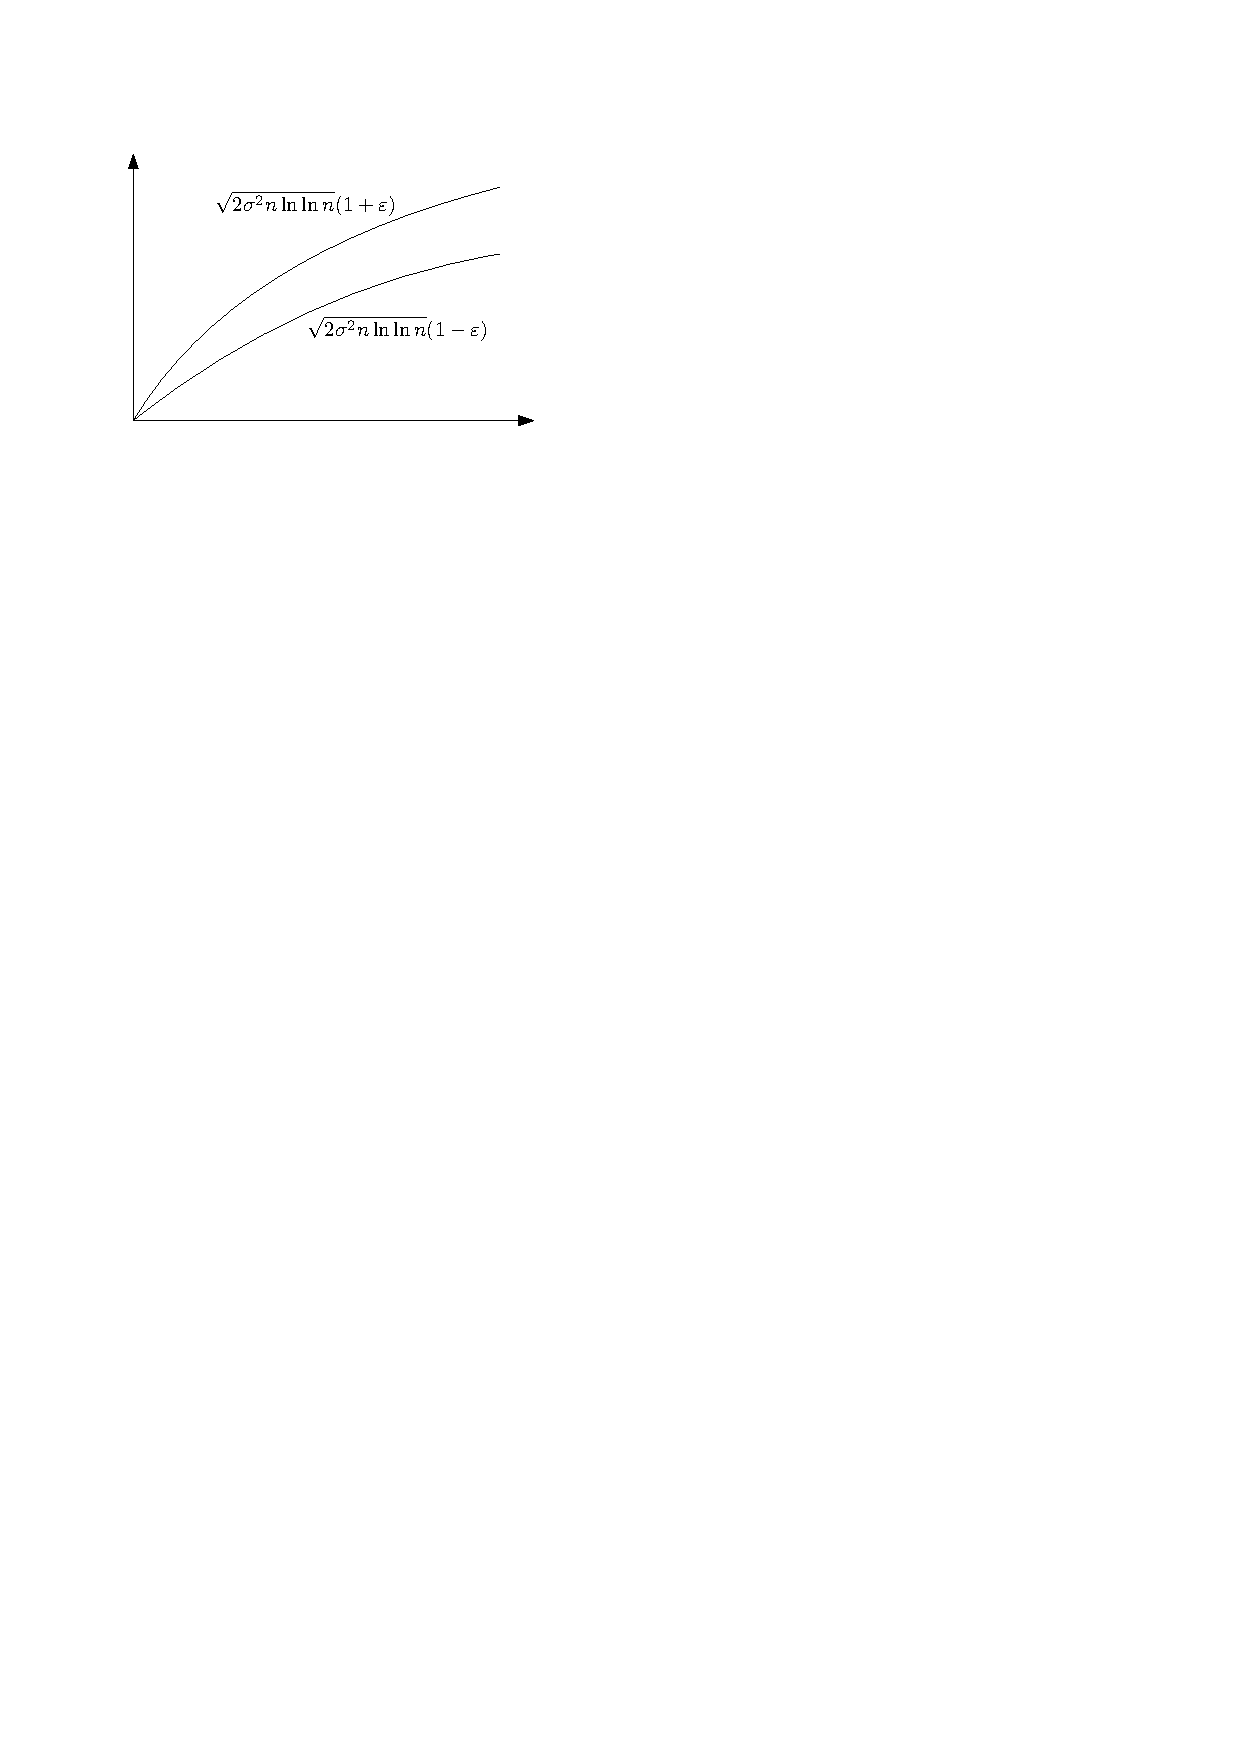
\includegraphics[width = 7cm]{lrl}
	\caption{Поведение верхней и нижней функции случайного блуждания}
	\label{pic:lrl}
\end{figure}
\subsection{Характеристические функции}
\begin{definition}
	Характеристическое функцией случайной величины $\xi$ называется $\varphi_\xi(t) = \E e^{it\xi}, t \in \R$.
\end{definition}
\begin{definition}
	Пусть $F(x)$~--- функция распределения, тогда ее характеристическая функция $\varphi_F (t) = \int\limits_\R e^{i t x} \, d F(x)$.
\end{definition}
 Если $F_\xi(x)$~--- функция распределения случайной величины $\xi$, то характеристические функции $\xi$ и $F_\xi$ совпадают.\\
 
 По формуле Эйлера $\varphi_\xi(t) = \E e^{i t \xi} = \E \cos (t \xi) + i \E \sin(t \xi)$.
 
 \begin{definition}
 	Пусть $\vec \xi = ( \xi_1, \ldots, \xi_n)$~--- случайный вектор. Его характеристической функцией называется $\varphi_{\vec \xi} \left(\vec t \right) = \E e^{i \left( \vec t, \vec \xi \right)}, t \in \R^n$.
 \end{definition}
 \begin{definition}
 	Пусть $F \left( \vec x \right), \vec x \in \R^n$~--- функция распределения в $\R^n$, тогда его характеристической функцией называется $\varphi_F \left( \vec t \right) = \int\limits_\R e^{i \left( \vec t, \vec x \right)} \, d F \left( \vec x \right), \vec x \in \R^n$.
 \end{definition}
 \subsection{Свойства характеристических функций}
 \setcounter{property}{0}
 \begin{property}
 	Пусть $\varphi(t)$~--- характеристическая функция случайной величины $\xi$, тогда $| \varphi (t) | \leqslant \varphi(0) = 1$.
 	\begin{proof}
 		$| \varphi(t) | = | \E e^{i t \xi} | \leqslant \E | \underbracket[0.5pt]{e^{i t \xi}}_{\equiv 1} | = 1 = \varphi(0)$.
 	\end{proof}
 \end{property}
	 







































	\section{Лекция от 28.04.2018}

	\begin{property}
		Пусть $\varphi(t)$~---характеристическая функция случайной величины $\xi$, а $\eta = a\xi + b$, где $a, b \in \mathbb{R}$, тогда $\varphi_\eta(t) = e^{itb}\cdot \varphi_\xi(at).$
		\begin{proof}
			$\varphi_\eta(t) = \E e^{it\eta} = \E e^{it(a\xi + b)} = e^{itb} \E e^{ita\xi} = e^{itb}\cdot \varphi_\xi(at).$
		\end{proof}
	\end{property}

	\begin{property}
		Пусть $\xi_1, \ldots, \xi_n$~---независимые случайные величины, $S_n = \sum\limits_{i = 1}^{n}\xi_i \Rightarrow \varphi_{S_n}(t) = \prod\limits_{i = 1}^n\varphi_{\xi_k}(t).$  
		\begin{proof}
			$\varphi_{S_n}(t) = \E e^{it \sum\limits_{k = 1}^{n}\xi_k} = \E\prod\limits_{k = 1}^n e^{it\xi_k} = \prod\limits_{k = 1}^{n}\E e^{it\xi_k} = \prod\limits_{k = 1}^{n}\varphi_{\xi_k}(t).$
		\end{proof}
	\end{property}
	\begin{property}
		Пусть $\varphi(t)$~--- характеристическая функция, тогда $\varphi(t) = \overline{\varphi(-t)}$
		\begin{proof}
			$\varphi(t) = \E e^{it\xi} = \E\overline{e^{-it\xi}} = \overline{\E e^{-it\xi}} = \overline{\varphi(-t)}.$
		\end{proof}
	\end{property}
	\begin{property}
		Пусть $\varphi(t)$~--- характеристическая функция случайной величины $\xi$, тогда $\varphi(t)$ равномерно непрерывна на $\mathbb{R}.$
		\begin{proof}
			Рассмотрим $|\varphi(t + h) - \varphi(t)| = |\E e^{i(t+h)\xi} - \E e^{it\xi}| = |\E e^{it\xi}(e^{ih\xi} - 1)| \leqslant \E |e^{it\xi}|\cdot |e^{ih\xi} - 1| = \E |e^{ih\xi} - 1|.$
			При $h \to 0$ выполнено $e^{ih\xi} - 1 \overset{\text{п.н.}} \longrightarrow 0 $ по теореме о наследовании сходимости. $\forall h: |e^{ih\xi} - 1| \leqslant |e^{ih\xi}| + 1 = 2, ~ \E 2 < +\infty$. Следовательно, по теореме Лебега о мажорируемой сходимости, $\E |e^{ih\xi} - 1| \to \E 0 = 0$. Значит, $\varphi(t)$ равномерно непрерывна.
		\end{proof}
	\end{property}
		\begin{theorem}[единственности (д-во позже)]
		Пусть $F$ и $G$~--- функции распределения, такие что $\varphi_{F(x)} = \varphi_{G(x)} \Rightarrow F(x) = G(x)~\forall x.$
	\end{theorem}
	\begin{property}
		Пусть $\varphi_\xi(t)$~---характеристическая функция случайной величины $\xi$, $\varphi(t)$ принимает действительные значения $\Leftrightarrow \xi$ имеет симметричное распределение.
		\begin{proof}
			$~(\Leftarrow)$ Пусть распределение $\xi$~---симметрично, тогда $E(\sin(t\xi)) = E(\sin(t(-\xi))) = -E(\sin(t\xi)) = 0.$ Значит $\varphi_\xi(t) = E\cos t\xi + iE\sin t\xi = E\cos t\xi \in \mathbb{R}.$

			$(\Rightarrow)$ Пусть $\varphi_\xi(t) \in \mathbb{R} ~\forall t.$ Тогда по свойствам $2$ и $3$ $\varphi_\xi(t) = \overline{\varphi_\xi(-t)} = \varphi_\xi(-t) = \varphi_{-\xi}(t) ~\Rightarrow $~$\xi$ и $-\xi$ имеют одиаковую характеристическую функцию $~\Rightarrow$~ $\xi \overset{d}{=} -\xi$ по теореме единственности.
		\end{proof}
	\end{property}

	\begin{property}
	\begin{theorem}[о производных х.ф.]
		Пусть $E|\xi|^n < + \infty, ~n \in \mathbb{N}.$ Тогда $\forall k \leqslant n~ \exists \varphi_\xi^{(k)}(t),$ причём
		\begin{enumerate}
			\item $\varphi_\xi^{(k)}(t) = \int\limits_\mathbb{R}(ix)^ke^{itx}dF(x)$
			\item $E\xi^k = \frac{\varphi_\xi^{(k)}(0)}{i^k}$
			\item $\varphi_\xi(t) = \sum\limits_{k = 0}^{n} \frac{(it)^k}{k!}E\xi^k + \frac{(it)^n}{n!}\varepsilon_n(t)$
		\end{enumerate}
		$|\varepsilon_n(t)| \leqslant 3E|\xi|^n, ~\varepsilon_n(t) \to 0, ~ t \to 0.$
	\end{theorem}
	\begin{proof}
		\begin{enumerate}
			\item Рассмотрим $\frac{\varphi_\xi(t + h) - \varphi_\xi(t)}{h} = \frac{Ee^{i(t + h)\xi} - Ee^{it\xi}}{h} = \frac{Ee^{it\xi}(e^{ih\xi} - 1)}{h}.$ при $h \to 0$ $\frac{e^{ih\xi} - 1}{h} \overset{\text{п.н.}}{\longrightarrow}i\xi,$ кроме того, $\left|\frac{e^{ih\xi} - 1}{h}\right| \leqslant |\xi|$ почти наверное, так как хорда меньше дуги. По теореме о мажорируемой сходимости
			$\lim\limits_{h \to 0}E \frac{e^{ih\xi} - 1}{h}e^{it\xi} = \varphi'_\xi(t) = E(i\xi\cdot e^{it\xi}) = \int\limits_\mathbb{R} ixe^{itx}dF_\xi(x).$ Доказательство формулы для $\varphi^{(k)}$ аналогично.
			\item Из пункта 1, $E\xi^n = \int\limits_\mathbb{R}x^k dF_\xi(x) = \frac{1}{i^k} \int\limits_\mathbb{R}(ix)^ke^{i0x}dF(x) = \frac{\varphi^{(k)}(0)}{i^k}.$
			\item Ряд Тейлора $e^{i\eta} = \sum\limits_{k = 0}^{n - 1} \frac{(i\eta)^k}{k!} + \frac{(i\eta)^n}{n!}(\cos\theta_1y + i\sin\theta_2 y), ~|\theta_1| \leqslant 1, ~ |\theta_2| \leqslant 1,$ тогда
			$\varphi_\xi(t) = Ee^{it\xi} = E\left[\sum\limits_{k = 0}^{n - 1} \frac{(it\xi)^k}{k!} + \frac{(it\xi)^n}{n!}(\cos\theta_1 t\xi + i\sin \theta_2 t\xi)\right] = \sum\limits_{k = 0}^{n}\frac{(it)^k}{k!}E\xi^k + \frac{(it)^n}{n!}\varepsilon_n(t), $ где $\varepsilon_n(t) = E(\xi^n\cdot [\cos\theta_1t\xi + i\sin(\theta_2 t\xi) - 1]) \Rightarrow \varepsilon_n(t) \leqslant 3E|\xi|^n;$

			$|\xi^n[\cos(\theta_1t\xi) + i\sin(\theta_2t\xi) - 1]| \leqslant3|\xi|^n$ и $\xi^n(\cos(\theta_1t\xi) - 1 + \underbrace{\sin(\theta_2 t\xi)}_{\to 0}) \overset{\text{п.н.}}{\longrightarrow} 0$ при $t \to 0 \Rightarrow$ по теореме Лебега о мажорируемой сходимости, $\varepsilon_n(t) \underset{t \to 0}{\longrightarrow} 0.$
		\end{enumerate}
	\end{proof}
	\end{property}
	\begin{property}[б/д]
		Если существует и конечна $\varphi^{(2n)}(0),$ то $E|\xi|^{2n} < +\infty.$
	\end{property}
	\begin{theorem}[о разложении х.ф. в ряд]
		Пусть $\xi$ случайная величина, такая что $E|\xi|^n < +\infty~ \forall n.$ Если для некоторого $T > 0$ выполнено $\overline{\lim\limits_{n}}\left(E \frac{|\xi|^n}{n!}\right) < \frac{1}{T},$ то $\forall t: |t| < T$ выполнено $\varphi_\xi(t) = \sum\limits_{n = 0}^{+\infty} \frac{(it)^n}{n!}E\xi^n.$
		\begin{proof}
			Пусть $t_0$ такое, что $|t_0| < T, $ тогда $\overline{\lim\limits_{n \to +\infty}}E\left(\frac{|\xi|^n \cdot |t_0|^n}{n!}\right)^{\frac{1}{n}} = \frac{|t_0|}{T} < 1, $ следовательно, по признаку Коши-Адамара сходимости рядов, ряд $\sum\limits_{n = 0}^{+\infty} \frac{E|\xi|^n\cdot|t_0|^n}{n!}$ сходится.
			Рассмотрим $|t| \leqslant |t_0|: \varphi_\xi(t) = \sum\limits_{k = 0}^{n} \frac{(it)^k}{k!}E\xi^k + \underbrace{\frac{(it)^n}{n!}\varepsilon_n(t)}_{R_n(t)}~~~(*).$ 

			\noindent$R_n(t) \leqslant 3\cdot \frac{|t|^n}{n!}\cdot E|\xi|^n \underset{n \to +\infty}{\longrightarrow} 0$ по условию теоремы. Устремляя $n\to + \infty$ в $(*)$, получаем $\varphi_\xi(t) = \sum\limits_{k = 0}^{+\infty} \frac{(it)^k}{k!}E\xi^k.$ В силу произвольности $|t_0| < T,$ разложение верно $\forall t \in (-T, T).$
		\end{proof}
	\end{theorem}

	\begin{example}
		Пусть $\xi \sim N(0;1) \Rightarrow \varphi_\xi(t) = e^{- \frac{t^2}{2}}.$ Мы знаем, что $E\xi^m = \left\{
			\begin{array}{l}
			(m-1)!!, ~m \vdots 2\\
			0, ~m\not \vdots 2
			\end{array}
		\right.$
		$E|\xi|^m = \left\{
			\begin{array}{l}
			(m - 1)!!, ~m \vdots 2\\
			(m - 1)!!\sqrt{\frac{2}{n}}, m \not \vdots 2
			\end{array}
		\right. \Rightarrow$ по предыдущей теореме, 
		$\varphi_\xi(t) = \sum\limits_{n = 0}^{\infty} \frac{(it)^{2n}}{(2n)!}(2n - 1)!! = \sum\limits_{n = 0}^{+\infty} \frac{(it)^{2n}}{(2n)!!} = \sum\limits_{n = 0}^{+\infty} \left(- \frac{t^2}{2}\right)^n \frac{1}{n!} = e^{-\frac{t^2}{2}}.$

		\underline{\text{Условие теоремы}}: $\left(\frac{E|\xi|^m}{m!}\right)^{\frac{1}{m}} \leqslant \left(\frac{(m - 1)!!}{m!}\right)^{\frac{1}{m}} = \left(\frac{1}{m!!}\right)^{\frac{1}{m}} \approx \frac{1}{\sqrt{2}}\left(\left(\frac{m}{2e}\right)^{\frac{m}{2}}\right)^{\frac{1}{m}} \sim \frac{C}{\sqrt{m}} \to 0 \Rightarrow T = + \infty.$
	\end{example}

	\begin{theorem}[формула обращения (б/д)]
		Пусть $\varphi(t)$ характеристическая функция функции распределения $F$. Тогда
		\begin{enumerate}
			\item Для $\forall a < b$ (точки непрерывности) $F$ выполнено
			$F(b) - F(a) = \frac{1}{2\pi} \lim\limits_{c \to +\infty} \int\limits_{-c}^{c} \frac{e^{-itb} - e^{-ita}}{-it}\varphi(t)dt$
			\item Если $\int\limits_\mathbb{R}|\varphi(t)|dt < +\infty,$ то у функции распределения $F(x)$ существует плотность $f(x)$ и $f(x) = \frac{1}{2\pi}\int\limits_\mathbb{R} e^{-tx}\varphi(t)dt.$
		\end{enumerate}
	\end{theorem}
	
	\section{Лекция от 05.05.2018}
	\begin{theorem}[единственности]
		Пусть \(F\) и \(G\)~--- функции распределения, такие что \(\varphi_{F(x)} = \varphi_{G(x)} \Rightarrow F(x) = G(x)~\forall x.\)
	\end{theorem}
	\begin{proof}
		Пусть \(a < b \in \mathbb{R}\). Рассмотрим \(f_\varepsilon(x)\)(шапочка). Докажем, что \(\forall \varepsilon > 0 \int\limits_{\mathbb{R}} f_\varepsilon(x) df(x) = \int\limits_\mathbb{R}f_\varepsilon(x)dG(x).\) Рассмотрим отрезок \([-n, n]\) такой, что \([a, b + \varepsilon] \subset [-n, n].\) По теореме Вейерштрасса-Стоуна, \(f_\varepsilon(x)\) сколь угодно точно приближается тригонометрическими многочленами от \(\frac{\pi x}{n}\), так как \(f_\varepsilon(x)\) непрерывна и периодична на \([-n, n]\) с периодом \(2n.\)

		\noindent \(\Rightarrow \forall n ~ \exists f_\varepsilon^n(x) = \sum\limits_{k \in K} a_k\cdot e^{\frac{ik\pi x}{n}}, ~a_k \in \mathbb{R},\) \(K\)~--- конечное подмножество \(\mathbb{Z},\) такое, что \(\forall x \in [-n, n]: |f_\varepsilon^n(x) - f_\varepsilon(x)| < \frac{1}{n}.\) \(f_\varepsilon^n\)~---периодическая с периодом \(2n.\) Поскольку \(|f_\varepsilon(x)| < 1\) и \(\forall x \in [-n, n]: |f_\varepsilon^n(x) - f_\varepsilon(x)| < \frac{1}{n}\), то \(|f_\varepsilon^n(x)| \leqslant 2 ~ \forall x.\) По условию, \(\int e^{itx}dF(x) = \int e^{itx}dG(x) \Rightarrow \int f_\varepsilon^n(x)dF(x) = \int f_\varepsilon^n(x)dG(x).\)
		\begin{gather*}
			\left|\int\limits_\mathbb{R} f_\varepsilon(x) dF(x) - \int\limits_\mathbb{R} f_\varepsilon(x)dG(x)\right| \leqslant \left|\int\limits_\mathbb{R} f_\varepsilon(x) dF(x) - \int\limits_\mathbb{R} f_\varepsilon^n(x) dF(x)\right| +\\
			+  \left|\int\limits_\mathbb{R} f_\varepsilon^n(x) dF(x) - \int\limits_\mathbb{R} f_\varepsilon^n(x) dG(x)\right| + \left|\int\limits_\mathbb{R} f_\varepsilon^n(x) dG(x) - \int\limits_\mathbb{R} f_\varepsilon(x) dG(x)\right| \leqslant\\
			\leqslant \frac{1}{n} \int\limits_{[-n,n]}dF(x) + \frac{1}{n} \int\limits_{[-n,n]}dG(x) +(\underbracket{1 - F(n)}_{\to 0} + \underbracket{F(-n)}_{\to 0} + \underbracket{1 - G(n)}_{\to 0} + \underbracket{G(-n)}_{\to 0}) \leqslant\\
			\leqslant \frac{2}{n} + o(1) \Rightarrow \forall \varepsilon> 0: \int f_\varepsilon(x) dF(x) = \int f_\varepsilon(x)dG(x).
		\end{gather*}
		При \(\varepsilon \to 0 f_\varepsilon(x) \to I_{[a,b]}(x),\) при этом \(|f_\varepsilon(x)| \leqslant 1~ \forall x \in \mathbb{R}.\) По теореме Лебега о мажорировании сходимости(рассматриваем \(f_\varepsilon(x)\) как набор случайных величин на \((\mathbb{R}, \B(\R), P_f) \to (\mathbb{R}, \B(\mathbb{R}))\)).
		\(\int\limits_\R f_\varepsilon(x)dF(x) \to \int\limits_\R I_{[a,b]}dF(x) = F(b) - F(a).\)
		Аналогично, для функции распределения \(G\) \(\int\limits_\R f_\varepsilon(x)dG(x) \underset{\varepsilon \to 0}{\longrightarrow} G(b) - G(a) \Rightarrow \forall a < b ~ F(b) - F(a) = G(b) - G(a).\)  Полагая \(a = (-\infty), \) получаем требуемое.
	\end{proof}

	\begin{theorem}[критерий назависимости]
		Пусть \(\vec{\xi} = (\xi_1, \ldots, \xi_n).\) Тогда \((\xi_1, \ldots, \xi_n)\)~--- назависимые в совокупности \(\Leftrightarrow \varphi_{\vec{\xi}(\vec{t})} = \prod\limits_{i = 1}^n \varphi_{\xi_i}(t_i) ~\forall \vec{t} = (t_1, \ldots, t_n) \in \R^n.\)
	\end{theorem}

	\begin{proof}
		\((\Rightarrow) ~ \varphi_{\vec{\xi}(\vec{t})} = Ee^{i(\vec{t}, \vec{\xi}}) = Eei^{\sum\limits_{k = 1}^{n}t_k\xi_k} \overset{\text{нез-сть}}{=} \prod\limits_{k = 1}^n Ee^{it_k\xi_k} = \prod\limits_{k = 1}^n \varphi_{\xi_x}(t_k).\)

		\((\Leftarrow)\) Пусть \(F_k(x)\)~--- функция распределения случайной величины \(\xi_k.\) Пусть \(G(x_1, \ldots, x_n) = F_1(x)\cdot\ldots\cdot F_n(x)\)~--- это функция распределения. Посчитаем её характеристическую функцию:
		\(\varphi_G(t) = \int\limits_{\R^n}e^{i(\vec{t}, \vec{x})}dG(\vec{x}) = \int\limits_\R e^{i(\vec{t}, \vec{x})}dF_1(x_1)\cdot\ldots\cdot dF_n(x_n) = \)(по теореме Фубини) \(\prod\limits_{k = 1}^n \int\limits_\R e^{it_kx_k} dF_k(x_k) = \prod\limits_{k = 1}^n\varphi_{\xi_k}(t_k) \overset{\text{по усл}}{=}\varphi_{\vec{\xi}}(\vec{t}) \Rightarrow\) характеристическая функция \(G\) и \(\vec{\xi}\) совпадают \(\Rightarrow\) по теореме единственности \(F_\xi = G \Rightarrow F_{\vec{\xi}}(\vec{x}) = \prod\limits_{k = 1}^n F_{\xi_k}(x_k) \Rightarrow \xi_1, \ldots, \xi_n\) независимы в совокупности по критерию независимости в терминах функции распределения.
	\end{proof}

	\subsection{Проверка того, что \(\varphi\)~---характеристическая функция}

	\begin{definition}
		Функция \(\varphi(t)\) является неотрицательно определённой, если \(\forall n ~ \forall t_1, \ldots, t_n \in \R, ~\forall z_1, \ldots, z_n \in \mathbb{C}, ~ \sum\limits_{i, j = 1}^{n}\varphi(t_i - t_j)z_k\overline{z_j} \geqslant 0.\)
	\end{definition}

	\begin{theorem}[Бохнера-Хинчина]
		Пусть \(\varphi(t)\) такая, что \(\varphi(0) = 1\) и \(\varphi(t)\) непрерывна в нуле. Тогда \(\varphi(t)\)~---характеристическая функция \(\Leftrightarrow \varphi(t)\) неотрицательно определённая.
	\end{theorem}

	\begin{proof}
		\((\Rightarrow) ~ \varphi(t)\)~--- характеристическая функция, проверим неотрицательность:
		\begin{gather*}
			\forall t_1, \ldots, t_n \in \R~\forall z_1, \ldots, z_n \in \mathbb{C}\\
			\sum\limits_{j, k = 1}^{n}\varphi(t_j - t_k)z_j \overline{z_k} =
			\sum\limits_{j, k = 1}^{n}Ee^{i(t_j - t_k)\xi}z_j\overline{z_k} = \\
			= E \sum\limits_{k, k = 1}^{n}e^{it_j\xi}\cdot z_j \cdot \overline{e^{et_k\xi}}\cdot \overline{z_k} = E\left|\sum\limits_{j = 1}^{n} e^{it_j\xi}z_j\right|^2 \geqslant 0
		\end{gather*}
	
		\((\Leftarrow)\) [б/д]
	\end{proof}
	\begin{consequence}
		Если \(\varphi(t) = \psi(t)\)~--- характеристическая функция, \(\alpha \in (0, 1),\) то \(\alpha \varphi(t) + (1 - \alpha)\psi(t)\)~--- характеристическая функция.
	\end{consequence}
	\begin{proof}
		Все три условия из теоремы Бохнера-Хинчина выполнены.
	\end{proof}
	\begin{theorem}[Пойа(б/д)]
		Пусть непрерывная, чётная и выпуклая вниз на \((0; + \infty)\) функция \(\varphi(t)\) такова, что \(\varphi(t) \geqslant 0, ~ \varphi(0) = 1, ~\varphi(t) \underset{t \to +\infty}{\longrightarrow} 0\). Тогда \(\varphi(t)\)~---характеристическая функция.
	\end{theorem}

	\begin{example}
		Любая функция вида
		\begin{center}
			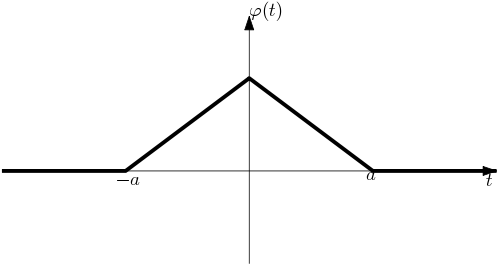
\includegraphics[scale=0.4]{img/img1.png}
		\end{center}
		является характеристической.
	\end{example}

	\begin{theorem}[Марцинкевича(б/д)]
		Если характеристическая функция \(\varphi(t)\) имеет вид ~\(\exp(P(t)),\) где \(P(t)\)~--- полином, то степерь этого полинома \(\leqslant 2 ~(\deg P(t) \leqslant 2).\)
	\end{theorem}
	\begin{example}
		\(e^{-t^n}\) не является характеристической функцией.
	\end{example}

	\begin{definition}
		Последовательность функций \(F_n(x)\) слабо сходится к \(F(x)\), если \(\forall f(x)\)~---  непрерывна и ограничена, то верно \(\int\limits_\R f(x) df_n(x) \to \int\limits_\R f(x)dF(x).\) Обозначение \(F_n \overset{w}{\longrightarrow}F.\)
		\((\xi_n \overset{d}{\longrightarrow}\xi \Leftrightarrow F_{\xi_n} \overset{w}{\longrightarrow}F).\)
	\end{definition}
	\begin{theorem}[нерперывности для х.ф.]~~~~~~~~~~~~~~~~~~~~~~~~~~~~~~~~~~~~~~~~~

		\noindent1. ~Пусть \(\{F_n\}_{n \geqslant 1}\)~--- последовательность функций распределения на \(\R\), тогда \(\varphi_n(t) \to \varphi(t) ~ \forall t \in \R, \) где \(\varphi\)~--- характеристическая функция \(F\).
		
		\noindent2.(б/д)~ Пусть \(\forall t \in \R ~ \exists \varphi(t) = \lim\limits_{n \to +\infty} \varphi_n(t), \) причём \(\varphi(t)\) непрерывна в нуле. Тогда \(\exists F\)~--- функция распределения такая, что \(F_n \overset{w}{\longrightarrow}F\) и \(\varphi\)~---характеристическая функция \(F\).
	\end{theorem}

	\begin{proof}
		Знаем, что  \(\forall f\)~--- непрерывной ограниченной функции : \(\int\limits_\R f(x)dF_n(x) \to \int\limits_\R f(x)dF(x).\) Но функции \(\sin tx \) и \(\cos tx\) непрерывны и ограничены \(\Rightarrow\) \(\varphi_n(t) = \int\limits_\R (\cos tx + i\sin tx)dF_n(x) \underset{n \to +\infty}{\longrightarrow} \int\limits_\R (\cos tx + i\sin tx)dF(x) = \varphi(t).\)
	\end{proof}

	\subsection{Центральная предельная теорема}
	\begin{theorem}[ЦПТ в форме Леви]
		Пусть \(\{\xi_n\}_{n\geqslant 1}\)~--- независимые одинаково распределённые случайные величины, \(0 < D\xi < +\infty.\)
		Обозначим \(S_n = \sum\limits_{i = 1}^{n}\xi_i.\) Тогда 
		\(\frac{S_n - ES_n}{\sqrt{DS_n}} \overset{d}{\underset{n \to +\infty}{\longrightarrow}}N(0, 1).\)
	\end{theorem}

	\begin{proof}
		Обозначим \(E\xi_i = a, D\xi_i = \sigma^2.\)
		Рассмотрим случайные величины \(\eta_i = \frac{\xi_i - a}{\sigma} \Rightarrow 
		E\eta_i = 0; ~ D\eta_i = 1.\)
		Тогда \(T_n = \frac{S_n - ES_n}{\sqrt{DS_n}} = \frac{S_n - na}{\sqrt{n\sigma^2}} = \frac{\eta_1 + \ldots + \eta_n}{\sqrt{n}}.\)
		Рассмотрим характеристическую функцию \(\eta_i\): по свойствам характеристической функции \(\varphi(t) \equiv \varphi_{\eta_i}(t) = 1 + it\underbracket{E\eta_j}_{0} + \frac{1}{2}\underbracket{E\eta_j^2}_1\cdot(it)^2 + o(t^2 = 1 - \frac{t^2}{2} + o(t^2), ~ t \to 0.\) Отсюда, \(\varphi_{T_n}(t) = \varphi_{\sum\limits_{j = 1}^{n}\eta_j}(t) \overset{\text{св-ва х.ф.}}{=} \left(\varphi\left(\frac{t}{\sqrt{n}}\right)\right)^n = \left(1 - \frac{t^2}{2} + o\left(\frac{t^2}{n}\right)\right)^n \underset{n \to \infty}{=} e^{- \frac{t^2}{2}}. \)Но \(e^{-\frac{t^2}{2}}\)~--- характеристическая функция \(N(0,1) \Rightarrow\) (по т. непрерывности) \(T_n = \frac{S_n - ES_n}{\sqrt{DS_n}} \overset{d}{\longrightarrow} N(0,1).\)
	\end{proof}
	\section{Лекция от 12.05.2018}

	\section{Лекция от 19.05.2018}
\begin{statement}[6-ое свойство]
	Если $\vec \xi \sim N(\vec m, \Sigma)$ и $\rg(\Sigma) = n$, то $\vec \xi$ имеет плотность в $\R^n$.
	\begin{proof}
		Так как $\rg \Sigma = n \Rightarrow \exists A = \Sigma^{-1}$. Обозначим $f(x) = \frac{|A|^{1/2}}{(2n)^{n / 2}} e^{-\frac{1}{2}(A(x - m), (x - m)), \vec x \in \R^n}$. Достаточно показать, что $\int\limits_{\R^n}e^{i(\vec t, \vec x)}f(x)dx = e^{i(\vec t, \vec m) - \frac{1}{2}(\Sigma \vec t, \vec t)}$, тогда $f$ --- плотность $\vec \xi$. Обозначим $I_n = \int\limits_{\R^n}e^{i(\vec f, \vec x - \vec m)} \frac{|A|^{1/2}}{(2\pi)^{n/2}}e^{-\frac{1}{2}A(\vec x - \vec m, \vec x - \vec m)}dx$. Хотим доказать, что $I_n = e^{-\frac{1}{2}(\Sigma\vec t, \vec t)}$. Мы знаем, что $\exists S$ --- ортогональная, такая что 
		$$ S^T\Sigma S = D = \left(\begin{matrix}
		d_1 & \ldots & 0 \\
		\vdots & \ddots & \vdots \\
		0 & \ldots & d_n \\
		\end{matrix}\right), d_i > 0, $$ 
		так как $\Sigma$ не вырожденная, тогда $|A| = |\Sigma^{-1}| = \frac{1}{d_1\cdot\ldots\cdot d_n}$. Сделаем замену: $\vec x - \vec m = S\vec u; \vec t = S\vec v$. Тогда $i(\vec t, \vec x - \vec m) - \frac{1}{2}(A(\vec x - \vec m), \vec x - \vec m) = i(S\vec v, S\vec u) - \frac{1}{2}(AS\vec u, S\vec u) = i\vec v^T\underbrace{S^TS_n}_{E_n} - \frac{1}{2}\vec u^T\underbrace{S^TAS}_{D^{-1}}u = i\vec v^T \vec u - \frac{1}{2}\vec u^TD^{-1}\vec u$. В итоге, 
		\begin{multline*}
		I_n = \frac{1}{(2\pi)^{n/2}(d_1 \cdot\ldots\cdot d_n)^{1/2}}\int\limits_{\R^n} e^{i(\vec v, \vec u)- \frac{1}{2}\vec u^TD^{-1}\vec u} \cdot J  \cdot du = \\
		= \prod\limits_{k = 1}^n\frac{1}{(2\pi d_k)^{1/2}} \int\limits_\R e^{i v_ku_k - \frac{1}{2}\frac{u_k^2}{d_k}}du_k = \prod\limits_{k = 1}^n e^{\frac{-v_k^2d_k}{2}} =  \\
		= e^{-\frac{1}{2}\vec v^TD\vec v} = e^{-\frac{1}{2}\vec v^TS^T\Sigma S\vec v} = e^{-\frac{1}{2}\vec t^T \Sigma t},
		\end{multline*} где $J = |S| = 1$ --- якобиан.  $e^{-\frac{1}{2}\vec t^T \Sigma t}$ --- характеристическая функция $\vec \xi \Rightarrow$ $f(x)$ --- плотность $\vec \xi$.
	\end{proof}
\end{statement}
\subsection{Многомерная ЦПТ}
\begin{theorem}[Многомерная ЦПТ]
	Пусть $|\vec x_i|_{i \geqslant 1}$ --- независимые одинаково распределенные случайные вектора, $\E\vec x_i = \vec a$, $\var \vec x_i = \Sigma$, тогда $\sqrt n \left( \frac{\vec x_1 + \ldots + \vec x_n}{n} \rightarrow \vec a \right) \xrightarrow{d} N(\vec 0, \Sigma),\; n \rightarrow +\infty$.
\end{theorem}
\begin{note}
	Сходимость векторов по распределению вводится аналогично обычной сходимости случайной величины по распределению, то есть $\forall f: \R^n \rightarrow \R$ непрерывно ограниченных $\E f(\vec x_n) \rightarrow \E f(\vec x)$.
	\begin{proof}
		Рассмотрим характеристическую функцию $\varphi_{k, n}(t) = \E \exp\left(i\left(t, \frac{x_k - a}{\sqrt n}\right)\right)$ и $\varphi_n(t) = \E \exp\left(i\left( \frac{S_n - na}{\sqrt n}, t \right)\right) = \prod\limits_{k = 1}^n\varphi_{k,n}(t)$, где $S_n = \sum\limits_{k = 1}^n \vec x_k$. Для доказательства достаточно убедиться, что $\varphi_n(t) \rightarrow e^{-\frac{1}{2}}\vec t^T\Sigma \vec t$. Заметим, что $\varphi_{k, n}(t) = \varphi_\xi\left( \frac{1}{\sqrt n} \right)$, где $\xi = (\vec x_k - \vec a, \vec t)$. Для $\varphi_\xi(S)$ верно представление (по теореме о производной характеристической функции) $\varphi_\xi(S) = 1 + S\varphi_\xi'(0) + \frac{S^2}{2}\varphi_\xi''(0) + o(S^2), S \rightarrow 0. \E \xi = 0, \D \xi = \E \xi \cdot \xi = \vec t^T \E(\vec x_k - \vec a)(\vec x_k - \vec a)^T\vec t = \vec t^T \Sigma \vec t \Rightarrow \varphi_\xi(S) = 1 - \frac{S^2}{2}\vec t^T\Sigma t + o(S^2), S \rightarrow 0 \Rightarrow \varphi_{k, n}(t) = \varphi_\xi\left(\frac{1}{\sqrt n}\right) = 1 - \frac{\vec t^T\Sigma \vec t}{2n} + o(\frac{1}{n}), n \rightarrow \infty$. Тогда $\varphi_n(t) = \prod\limits_{k = 1}^n\varphi_{k, n}(t) = \left( 1 - \frac{1}{2n}\vec t^T\Sigma\vec t + o\left( \frac{1}{n} \right) \right)^n \limn \exp\left( -\frac{1}{2}\vec t^T \Sigma t \right)$.
	\end{proof}
\end{note}
\end{document}	